\chapter{Dependent Mixtures: Modelling Cell Lineages}
\label{ch:cell_lineage}
\index{Instructions for Preparing Dissertations, Theses, and Reports%
@\emph{Instructions for Preparing Dissertations, Theses, and Reports}}%


\section{Introduction}

This chapter introduces a Bayesian mixture model with dependent prior on the
component-specific parameters.
The simplest Bayesian mixture models assume independent
priors on cluster-specific parameters that index the sampling model
for each term of the mixture model, motivated mostly by ease of implementation.
For a review of Bayesian inference in mixture models see, for example, \citet{fruhwirth2006finite} and \citet[Chapter 1]{handbookmixtures2019}. 

However, in many situations, the observed data structure is not well supported by independent mixture components.
\citet{xu2016bayesian} argue for priors that favor diverse and parsimonious components in the mixture via determinantal point process. 
The idea is to favor mixture models with terms that define meaningfully different subpopulations. 
This becomes important if the inference aim is related to a biological interpretation of the underlying structure. 
While one can argue that asymptotically posterior inference in mixtures will concentrate on a parsimonious structure \citep{rousseau2011asymptotic}, this is not true for any finite sample size unless appropriate model assumptions are explicitly introduced.
In this paper we consider an inference problem that gives rise to a special type of parsimony in a mixture model.


\subsection{Modeling cell lineage data}
\label{sec:intro_cell_lineage}
The work developed in this chapter is motivated by the study of cell lineages. Cell lineage data comes from single-cell transcriptomics and it is used to recover the evolutionary path of cells in a given environment.
The finer resolution of single-cell assays such as single cell RNA sequencing experiments (scRNAseq) in comparison with aggregated "bulk" data provides cell-specific data. Applications include for example studies in immune systems \citep{stubbington2017single,miragaia2017single}, virus-host interactions \citep{cristinelli2018use}, hematopoiesis \citep{wilson2018single,dharampuriya2017tracking} among others. 
In particular, single-cell assays allow to trace back the ``history'' of fully differentiated cells starting from their precursors, so they have become very important to the study of cell lineages \citep{stubbington2017single}.

A typical cell lineage dataset contains a sample of cells from a certain tissue along with cell-specific transcriptional profiles obtained, for example, from scRNAseq. 
Such profiles exhibit differences that are associated with the development stage of the cell. 
For instance, stem cells evolve into fully differentiated cells according to a process characterized by gradual transcriptional changes. Therefore, important differences are observed in transcription profiles along the development path of the cell. 
Another potential application concerns temporal transformation of the cells, e.g. during cancer progression. 
Lineage inference is then carried out to identify the underlying path of development from the initial state of the cell until its matured states. 
For a more detailed description of the objectives and challenges of lineage inference, see \cite{korthauer2016statistical} .


%\begin{figure}[!ht]
%	\centering
%	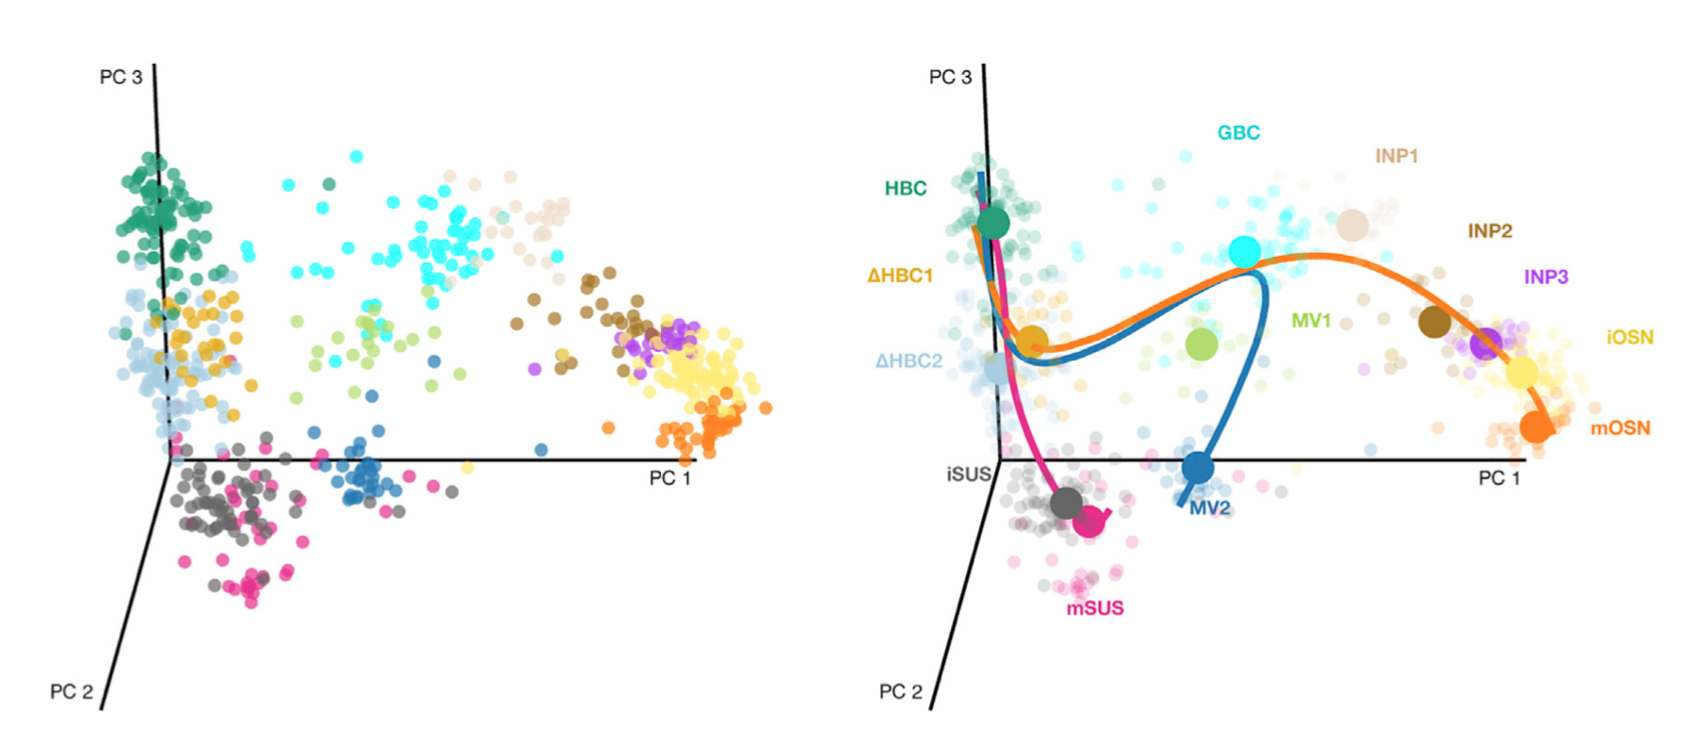
\includegraphics[width=.85\linewidth]{./Img/sample_data}
%	\caption{Left panel: Three-dimensional representation of single-cell gene expression profiles based on principal component analysis (data of \cite{fletcher2017deconstructing}); cells are colored by cluster. Right panel: results using the ``Slingshot'' method of \cite{street2018}.}
%	\label{fig:ex_data}
%\end{figure}


\begin{figure}[!ht]
	\centering
	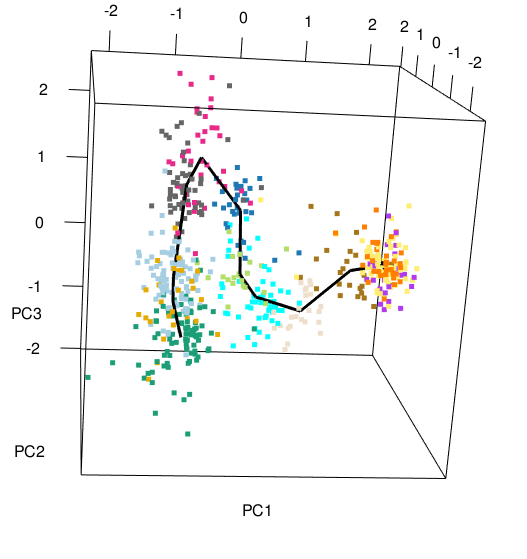
\includegraphics[width=.4\linewidth]{./Img/fletcher/fletcher_data_3d.png}
	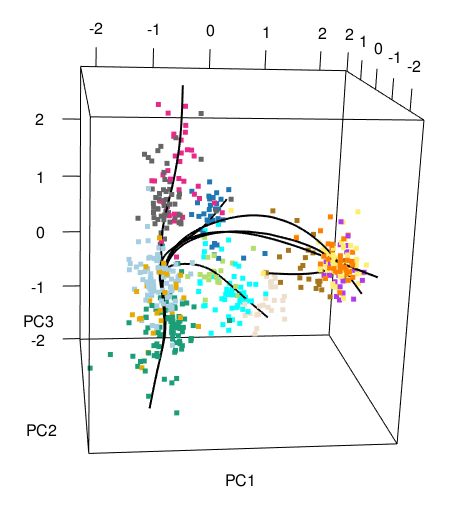
\includegraphics[width=.4\linewidth]{./Img/fletcher/fletcher_data_slingshot.png}	
	\caption{Left panel: Three-dimensional representation of single-cell gene expression profiles based on principal component analysis (data of \cite{fletcher2017deconstructing}); cells are colored by cluster. Right panel: results using the ``Slingshot'' method of \cite{street2018}.}
	\label{fig:ex_data}
\end{figure}

Typically, the process of estimating the latent tree in cell lineage problems is done in three sequential steps. First,  dimension reduction methods are applied to summarize information from the high dimensional scRNAseq data; then clustering of the cells is carried out in the reduced dimensional space; finally, the latent tree is inferred given the estimates of the partition of cells. Figure \ref{fig:ex_data} illustrates the results of this sequential approach applied to a lineage cell lineage dataset. Notice how in Figure Figure \ref{fig:ex_data} (and the following discussion) the data includes observations on all nodes of the tree, not only the leaves. This is because the data is a snapshot of cells accross all intermediate steps in the evolution of the cells.

\cite{Shiffman18} introduce a generative model based on a Dirichlet diffusion process \citep{neal:03}. 
This model, however, despite introducing a notion of tree along which cell evolution occurs, the model does not favor simple trees with well dinstinguished clusters of cell. Trees from a Dirichlet diffusion process are generated on a latent space via Brownian motion and thus do not enforce neither a partition nor a parsimonious representation of the data. 

In contrast, \cite{street2018} develop a method (``Slingshot'') that takes as input a partition of the cell lines into different cell types and returns a smooth version of the underlying MST defined by the clusters' centroids: the paths from root to leaves are smoothed by principal curves. The Slingshot procedure requires observations to be clustered, which is done sequentially by a k-means algorithm for instance, before the construction of a minimum spanning tree on the cluster centroids. Such sequential approach (of first fixing the partition of cells, then using the centroids as nodes of the MST) is very common in the bioinformatics literature despite its assumption that the lineage structure (represented by the MST) does not play a role in clustering the cells. Such assumption is not biologically ideal.


In the following section we propose an inference approach that uses a model-based Bayesian perspective such as in \cite{Shiffman18}, but in the context of mixtures as in ``Slingshot''.
That is, we propose a Bayesian dependent mixture model for cell lineage inference. 
The mixture components represent clusters of cells in the same development stage and the dependence is defined by a latent random tree with nodes that correspond to the centroid of the clusters. The cluster and lineage structures are modeled jointly and as a consequence, the lineage represented by the random tree structure is allowed to affect the clustering of cells. 
Full posterior inference on the clusters, the random tree and pseudotimes are obtained by Markov chain Monte Carlo (MCMC). 


\subsection{Dependent mixture models}

The proposed model is a variation of Bayesian mixture models in which dependent priors are assumed. 
Clusters of cells should be dependent on each other due to the fact that mixture components represent distinct intermediate states in the continuous process of cell development. 
Most literature on Bayesian mixture models assumes a priori independent cluster-specific parameters, with some exceptions. 
\cite{xu2016bayesian} describe the application of determinantal point processes (DPP) \citep{dpp_original} in Bayesian mixture models as a way to impose repulsive stochastic behaviour for the prior on the mixture components. 
The motivation comes from the observation that similar mixture components do not make the model more flexible. 
Conversely, they only create redundancy and hurt the interpretability of the components. 
In the context of cell lineage data, the repulsive nature of the DPP would enforce the intermediate states of cell development to be dissimilar from each other.

Another motivation for dependent mixtures is the sharing of information between the different groups, causing a shrinkage effect that is also a form of regularization. 
Mixed effect models is a key example of the use of hyperpriors for regularization \citep{lindstrom1990nonlinear,alston2012bayesian,lachos2013bayesian}.
In Bayesian non-parametrics, hierarchical Dirichlet processes \citep{HDP} incorporate shrinkage effect by assuming dependent component-specific Dirichlet processes (DP) $G_j \sim DP(\alpha_0, G_0)$ for mixture components $j=1, \dots, K$ with a common base measure $G_0$ that is itself a DP. 
Since DPs generate discrete random measures with the countably infinite support consisting of an iid sample from the base measure, it follows from the discreteness of $G_0$ that all $G_j, \ j=1, \cdots, K$ will all share the same atoms.


An application of mixture models with predictor-dependent components is described in \cite{chung2011local}. 
The authors define a Dirichlet process that assigns stick-breaking weights and atoms to random locations in predictor space, therefore obtaining random probability measures (which define the distribution of the mixture components) indexed by covariates in a continuous way.
 

Our proposal is to define dependence on the components of the mixture in a way that explicitly incorporates the biological structure that characterizes cell lineage applications. 
We therefore propose the use of a random tree structure not only to explain the snapshot in the latent space of the continuous development of cells from its initial stage into mature differentiated cells, but also to model the dependence structure between the clusters of cells.
Regularization is incorporated in the form of a penalization on trees with too many nodes or with redundant edges. 
Our proposed model builds upon the slingshot model in \cite{street2018} in which a Minimum Spanning Tree is calculated given the estimated centroids of the clusters of cells in a latent low dimensional space. The authors then use projections onto the MST to get a point estimate of the pseudotimes for each cell. 
In contrast, by formally constructing a Bayesian mixture model with random trees on such latent space, we are able to provide full inference (with uncertainty captured by the posterior samples obtained through MCMC) on the clusters of cells, on the underlying tree structure and also on pseudotimes. In addition, the model assumes the partition of cells to depend on the lineage structure.

\section{Dependent  Mixture Models for Cell Lineage Data}


% \subsection{A Dependent Mixture Model}
Let $\bfy_i \in \mathbb{R}^D$ denote the recorded markers for the $i$th cell. 
In a study of cell lineage, the raw data could be biomarkers, i.e., protein levels for some selected proteins. 
The raw data are typically further processed by extracting, for example, the first few principal components which become the data $\bfy_i$ in the upcoming discussion.

We start the construction of a Bayesian inference model by assuming a mixture sampling model for $\bfy_i$, $i=1, \ldots, n$. 
Let $\bftheta$ denote all unknown parameters. 
We assume
\begin{equation}
	  \bfy_i \mid \bftheta \iid \sum_{j=0}^k w_j \ N(\bfy_i  \mid \bfmu_j, \Sigma_j).
	\label{eq:likelihood}
\end{equation}
The parameter vector $\th$ includes, in particular, the number of terms in the mixture, $k+1$, the location parameters $\bfmu_j$ and the covariance parameters for each cluster in the mixture model, and the relative weights $w_j$, $j=0, \ldots, k$.

In words, we assume a mixture of normals for the data $\bfy_i$, including cluster-specific covariance matrices $\Sigma_j$ and cluster-specific location parameters $\bfmu_j$.
Next, we introduce a dependent prior across $\bfmu_j$.
Dependence is supported by the nature of the cell subpopulations being biologically related as part of the cell differentiation process.


 Recall that the goal is  to infer a structure that reflects the cell evolution path and its possible branching,  starting with an original cell population indexed by $k=0$ (and biologically known to be the root population).
 We represent this cell evolution path as a tree that includes the terms $\bfmu_j$ in the mixture model \eqref{eq:likelihood} as the vertices, which are connected by edges that represent the cell differentiation.
An additional set $\bfb=(b_1, \ldots, b_k)$ of indicator variables $b_j \in \{0,\ldots,k\}$ records the tree structure by specifying for each node the index of the parent node. The root node, $j=0$ has no parent.
A prior on the tree implicitly defines the prior probability model for the mixture component locations $\bfmu_j$, as described in Sections \ref{sec:soft_mst} and \ref{sec:model2_mst}. 

In order to define a meaningful notion of cell evolution, we need to carefully choose the form of such tree.
This is achieved by defining a tree with a globally-dependent structure, which is able to induce repulsions between the branches and to avoid redundant components. 
For example, we avoid the possibility of a tree to grow back into itself. 
In fact, cell evolution follows a ``monotonicity'' requirement in the sense that cell characteristics evolve towards progressive degrees of differentiation, not going back to an undifferentiated stage.

 We introduce a preference for such structure using the notion of a minimum spanning tree (MST), whose origin traces back to \cite{boruuvka1926contribution}.
A MST is an edge-weighted, undirected graph that connects all vertices together, without any cycles and with the minimum possible total edge weight.  
The weight on an edge is  the distance between the two nodes of the corresponding edge. 
In such a way, the most likely tree induces the desired parsimony requirement. 
In fact, given a set of nodes representing the different cell subpopulations, a MST can be seen as the most parsimonious way to represent the cell lineage.


We consider two alternative priors for $(k,\bfmu_1,\ldots,\bfmu_k)$ based on a MST.
One model is centered around trees that constitute a MST of the locations $\bfmu_j$, but also allows trees that are not MST. 
The second model restricts the tree to be a MST, making $\bfb$ a deterministic function of $(\bfmu_0,\ldots,\bfmu_k)$.


\subsection{Soft MST-dependent prior}
% Mixture model of soft Minimum Spanning Trees
\label{sec:soft_mst}


Let $\mathcal{T}_k = (k, \bfmu_1, \dots, \bfmu_k, b_1, \dots, b_{k})$
denote the tree, including cluster locations $\bfmu_j$ (note that $\bfmu_0$ is known and hence no prior is assigned to it) and tree
structure $\bfb$.
The soft-MST (s-MST) prior defines a dependent prior on the cluster
locations as 
\begin{equation}
  p(\bfmu_1, \dots, \bfmu_k, \bfb, k) \propto \prod_{j=1}^k
  \left\{ q(\bfmu_j) \right\} \exp\left\{- \alpha \sum_{j=1}^k
    d^2(\bfmu_j, \bfmu_{b_j}) \right\} q(k).
\label{eq:prior1}
\end{equation}
with $\bfb$ restricted to tree structures, i.e., no cycles and a single known root in $\bfmu_0$. Also, notice that \eqref{eq:prior1} includes $k$ as a random variable.

In equation \eqref{eq:prior1}, $d(\bfmu_i, \bfmu_j)$ denotes the Euclidean distance between two nodes $\bfmu_i$ and $\bfmu_j$. The terms $q(k)$ and $q(\bfmu_j)$ are reference probability models. We use $q(\bfmu_j)\sim N(\bfmu_j \mid m_0, \sigma^2_0 I)$ where $I$ denotes the identity matrix of dimension $D$. The penalty parameter $\alpha$ controls the level of shrinkage towards a MST, with $\alpha=0$ implying no shrinkage and $\alpha \rightarrow \infty$ implying a deterministic restriction to MSTs. In summary, equation \eqref{eq:prior1} is the prior on the random tree. It is difficult to visualize $p(\mathcal{T}_k)$ by way of prior simulation.

It is important to notice that $q(k)$ and $q(\bfmu_j)$ are not the marginal models for $k$ and $\bfmu_j$. The marginal distributions are implicitly determined by $q(k)$, $q(\bfmu_j)$ and by the parameter $\alpha$. In fact, conditionally on $k$, the model in \eqref{eq:prior1} reduces to 
$$
p(\bfmu_1, \dots, \bfmu_k, \bfb | k) = \frac{1}{Z_{k}}
\prod_{j=1}^k \left\{ q(\bfmu_j) \right\} \exp\left\{- \alpha
  \sum_{j=1}^k d^2(\bfmu_j, \bfmu_{b_j}) \right\},
$$
where
$$
Z_{k} = \int \dots \int_{\mathbb{R}^{p \times k}} \prod_{j=1}^k \left\{
  q(\bfmu_j)\right\} \cdot \left[ \sum_{b_1=0}^k \dots
  \sum_{b_k=0}^k \exp\left\{- \alpha \sum_{j=1}^k d^2(\bfmu_j,
    \bfmu_{b_j}) \right\} \right] \ d\bfmu_1 \dots  d\bfmu_k
$$
is an intractable normalizing constant. The marginal prior on $k$ can
be written as $ p(k) \propto Z_{k} \ q(k)$ with normalization constant $\sum^{\infty}_{k=1} Z_{k} \ q(k)$. It is easy to see that $p(\bfmu_1, \dots, \bfmu_k, \bfb, k)$
defined in \eqref{eq:prior1} is proper (see Appendix
\ref{sec:proper_prior}).

The dependence among the centers is induced by the exponential term,
that penalizes complex branching structures; for example, in trees
with too many nodes or with redundant edges. Therefore, the prior can
be seen as a regularization term, that is ballanced by the
likelihood, which tends to favor complex trees that provide better
fit to the training data. The parameter $\alpha$ determines the
strength of the regularization implied by the prior in comparison with
the likelihood of the data. Implicit in \eqref{eq:prior1} is the fact
that the only branching structures $\bfb$ allowed are the ones that
span trees with no internal cycles.
% Notice that complex branching structures are allowed (albeit
% discouraged, unless the data suggest so), not restricting to the
% case of binary branching. 

%The dependency among the centers is induced by the exponential term,
%that penalizes branching structures that are redundant and not
%supported by the data.  
%Implicit in \eqref{eq:prior1} is the fact that the only branching
%structures $\bfb$ allowed are the ones that span a tree with
%vertices $\bfmu_1, \ldots, \bfmu_k$ having no cycles. Notice that
%complex branching structures are allowed (albeit discouraged, unless
%the data suggest so), not restricting to the case of binary
%branching. 

This joint prior, despite presenting an intractable normalizing
constant, induces simple conditionals. For example, note that  
\begin{multline}
  p(b_j = i | \bfmu_1, \dots, \bfmu_k, \bfb^{(-j)},  k)
  \propto \exp \left\{ - \alpha \ d^2(\bfmu_j, \bfmu_i) \right\},
  \\ \forall i = 0, \dots, k ,\ \forall j = 1, \dots, k 
  \label{eq:b_cond}
\end{multline}
and that 
\begin{equation}
  p(\bfmu_j | \bfmu^{(-j)}, \bfb, k) \propto q(\bfmu_j) \exp
  \left[ - \alpha \left\{ d^2(\bfmu_j, \bfmu_{b_j}) + \sum_{l : b_l
        = j} d^2(\bfmu_l, \bfmu_j) \right\} \right]. 
  \label{eq:mu_cond}
\end{equation}
Equations \eqref{eq:b_cond} and \eqref{eq:mu_cond} reflect the repulsive
effect of the prior on the branching structure.  In fact, the
conditional distribution for $\bfb$ favours minimum spanning trees
by assigning smaller probabilities to redundant structures,
e.g. branches that grow back.  This can be seen by the fact that each
branch is selected to be the shortest (with larger probabilities)
among those who preserve the spanning structure of the tree.  In the
case $\alpha \rightarrow +\infty$, this procedure has several
analogies with Prim's algorithm \citep[see][]{prim1957shortest}.  In
the opposite case, i.e. when $\alpha \rightarrow 0$, the prior on the
trees is invariant with respect to the branching structure and the
centers are independent.  The model in this case corresponds to a
finite mixture model with a prior on the number of components.  In
general, the model does a soft assignment of the branches to a MST
structure (s-MST).

The conditional prior on the means, instead has a different effect.
Each center is drawn from a linear combination of the independent
prior term and the position of its parent and children.  The larger
the $\alpha$ parameter, the more evident the attraction towards the
barycentre of parent and children.  Moreover, note that if the
distance $d$ chosen is the squared euclidean, the conditional
distribution of each $\bfmu_j$ is still normal, with updated
parameters, i.e.
\begin{align}
\bfmu_j | \bfmu^{(-j)}, \bfb, k &\sim \mathcal{N}\left( \bfmu_p, \Sigma_p\right),\nonumber \\ 
\bfmu_p &= \frac{\bm{m}_0/\sigma_0^2 + 2 \alpha (\bfmu_{b_j} + \sum_{l:b_l = j} \bfmu_l)}{1/\sigma_0^2 + 2 \alpha (1 + f_j)} \label{eq:mu_cond_eucl1} \\
\Sigma_p &= \left\{ \frac{1}{\sigma_0^2} + 2 \alpha (1 + f_j) \right\}^{-1} I.
\label{eq:mu_cond_eucl2}
\end{align}
where $f_j$ is the number of children of node $j$ and $(\bm{m}_0, \sigma_0^2)$ are the prior hyperparameters of $q(\bfmu_j)$. The Gaussian prior on $(\bfmu_j | \bfmu^{(-j)}, \bfb, k)$ is a fundamental feature that will imply posterior conditional conjugacy. 

For the weights and the kernel covariance we use conditionally conjugate priors, 
\begin{eqnarray}
	\Sigma_0, \dots, \Sigma_k & \sim & \IW\left( \nu, \Psi \right) \nonumber \\
	(w_0, \dots, w_k) \mid k &  \sim & \Dir(\delta, \dots, \delta) 	\label{eq:prior_cov}\\
	\alpha &\sim & \mbox{Exp}(\lambda_0) \nonumber\\
	k &\sim & \text{Geom}(k - 2 | r_0), \ k \geq 2. \nonumber
\end{eqnarray}


\subsection{Hard MST-dependent mixture model}
\label{sec:model2_mst}

% A special case of the model described in section \ref{sec:soft_mst} is
% obtained when the branches $b_j$ determine the minimum spanning tree
% with vertices $\bfmu_1, \ldots, \bfmu_k$. The MST structure is
% favoured when $\alpha \rightarrow +\infty$, although there is always a
% positive probability of sampling oher trees that are not the MST. In
% this section we show how a simple modification of the model described
% in section \ref{sec:soft_mst} can impose MST structure. We highlight
% that the resulting model is simpler to implement as it does not
% require sampling the branches $b_j$ while maintaining full
% conditionals in analitical form. The obvious drawback is the loss of
% flexibility in the branching structure. 

%(When should one prefer to enforce MST? )
The prior in \eqref{eq:prior1} formalizes a preference for parsimonious structure by favoring mixture models with clusters that are connected by a tree with short cumulative length. 
By favoring shorter cumulative length the model shrinks the tree structure towards a MST, but stops short of insisting on the tree actually being a MST. 
The model defines a joint prior $p(\bfmu,\bfb)$ on the cluster locations $\bfmu=(\bfmu_j)^k_{j=1}$ and the tree $\bfb$.
An alternative model, named here as hard-MST (h-MST), defines a prior on $\bfmu$ only and implies $\bfb$ by introducing the MST as a deterministic function $\bfb = \mbox{MST}(\bfmu)$ of $\bfmu$: 

\begin{equation}
  p(\bfmu_1, \ldots, \bfmu_k \mid k) \propto \prod_{j=1}^k
  \left\{ N(\bfmu_j; \ \bfm, \ \sigma^2_0I) \right\} \exp\left[ -\alpha
    \mathcal{W}\left\{ MST(\bfmu_1, \ldots, \bfmu_k) \right\} \right].
\label{eq:hMST}
\end{equation}

The term $\mbox{MST}(\bfmu_1, \ldots, \bfmu_k)$ in equation \eqref{eq:hMST} represents the minimum spanning tree with nodes $\bfmu_1, \ldots, \bfmu_k$ and edges $E_{\bfmu_1, \ldots, \bfmu_k} \subset \{1, \ldots, k\}^2$. The function $\mathcal{W}$ denotes the total length of a graph, which is defined by the sum of the squared lengths of its edges. Therefore, we have

$$\mathcal{W}(MST(\bfmu_1, \ldots, \bfmu_k)) = \sum_{(j_1, j_2) \in E_{\bfmu_1, \ldots, \bfmu_k}} d^2(\bfmu_{j1}, \bfmu_{j2}).$$

By taking the lengths of the edges squared to define the length of the whole tree, we preserve conjugacy for the component specific means. By enforcing the MST structure the h-MST model provides stronger parsimony (in terms of favoring simpler tree structures) if compared with the s-MST. The parameter $\alpha$ regulates the strength of influence of the MST on the clustering structure: the higher its value, the simpler the underlying tree structure due to a stronger penalization on the length of the MST.

Under the h-MST, the priors for the remaining parameters are the same as described in section \ref{sec:soft_mst} equation \eqref{eq:prior_cov} for the s-MST. 

As mentioned in subsection \ref{sec:intro_cell_lineage}, there is a crucial difference between our modeling approach and the two-step slingshot algorithm of \cite{street2018} with regards to the dependence relationship of the cell lineage and the cluster centroids. Although the hard MST-dependent mixture model defines the MST as a deterministic function of the cluster centers, it implies a regularization effect of the tree structure on the distribution of the centroids by favoring cluster-specific means that lead to simpler (shorter) MSTs. On the other hand, the clustering step in \cite{street2018} does not make use of the underlying lineage structure represented by the MST.

All full conditional distributions for this model are analytically available, except for $p(\bfmu_j\mid \bfy, \mbox{rest})$ for which a Mtropolis-Hastings step was implemented. More details are available in Appendix \ref{sec:app_hmst}.



\section{Posterior Inference}
\label{sec:mst_inference}

In this section, we present the posterior simulation scheme to infer the tree structure, the optimal clustering configuration, as well as the estimation of the pseudotimes for each cell. For both the s-MST and h-MST models, the inference procedure is done via reversible jumps MCMC. 


For inference with an unknown number of components $k$ we 
added a prior $k \sim \mbox{Geom}(k - 2 | r_0), \ k \geq 2$ and implement transdimensional  posterior simulation, to accommodate the variable dimension of the parameter vector as $k$ changes. The soft-MST prior uses reversible jump MCMC (RJ-MCMC) \citep{green1995}  to implement trans-dimensional transitions.  Proposing a tree also requires a proposal for the branching structure. However, given $k$ nodes the total number of spanning trees is $k^{k-2}$, implying a curse of dimensionality for even fairly moderate values of $k$.  This would in turn lead to inefficient proposals, which cause the algorithm to mix poorly.

In order to overcome this issue, we propose a variant of the RJ-MCMC
which has been previously used in \cite{xu2016bayesian} and
\cite{lee2015bayesian}.  Denote the parameters with
$\bm{\theta}_k = (\bfmu_1, \dots, \bfmu_k, b_1, \dots, b_k, w_0,
\dots, w_k, \Sigma_0, \dots, \Sigma_k)$.  In the RJ-MCMC, a proposal that involves a
change of $k$ to $\tilde{k}$ would require to propose also a new set
of parameters $\tilde{\bm{\theta}}_{\tilde{k}}$.  In practice, the
joint proposal for a ``new'' dimension and a ``new'' set of
parameters, decomposes in $q(\tilde{\bm{\theta}}_{\tilde{k}},
\tilde{k} | \bm{\theta}_{k}, k) = q(\tilde{\bm{\theta}}_{\tilde{k}} |
\tilde{k}, k, \bm{\theta}_{k})\ q(\tilde{k} | k)$. In practice, it is difficult to make good proposals $q(\tilde{\bftheta}_{\tilde{k}}, \tilde{k} \mid \bftheta_k, k)$ and $q(\bftheta_k, k \mid \tilde{\bftheta}_{\tilde{k}}, \tilde{k} )$ with reasonable acceptance probabilities. 

We follow an approach from \cite{lee2015bayesian} nd \cite{xu2016bayesian}.
The idea is to split the data into two parts: a small
training set $y^\prime$ that serves the purpose of creating
informative proposal distributions, and a test set $y^{\prime \prime}$
to evaluate the acceptance ratio.  Let $p_1(\bm{\theta}_k | y^\prime)
= p(\bm{\theta}_k | k, y^\prime)$ denote the posterior distribution
under $k$ using the training sample $y^\prime$.  We use $p_1$ in two
instances.  First, we replace the original prior term $p(\bm{\theta}_k
| k)$ and, second, we also use it as proposal distribution
$q(\tilde{\bm{\theta}}_{\tilde{k}} | \tilde{k})$.  The test data
$y^{\prime \prime}$ is then used to evaluate the acceptance
probability.  By the nature of the Metropolis-Hastings acceptance
probability the proposal distribution and the prior factor in the
target distribution cancel out, making this a feasible strategy, i.e.
\begin{align}
\alpha(\tilde{\theta}_{\tilde{k}}, \tilde{k}\mid \theta_k, k) &= \min \left\{ 1; \frac{p(\tilde{k}) \ p (y^{\prime \prime} | \tilde{\bm{\theta}}_{\tilde{k}}, \tilde{k}) \cancel{p_1(\tilde{\theta}_{\tilde{k}} \mid \tilde{k})}\ \bcancel{q(\theta_k | k)} q(k | \tilde{k}) }{p(k) \ p (y^{\prime \prime} | \bm{\theta}_k, k) \ \bcancel{p_1(\theta_k \mid k)} \ \cancel{q(\tilde{\theta}_{\tilde{k}} \mid \tilde{k})} \ q(\tilde{k} | k)} \right\} \nonumber \\
&=\min \left\{ 1; \frac{p(\tilde{k}) \ p (y^{\prime \prime} | \tilde{\bm{\theta}}_{\tilde{k}}, \tilde{k})\ q(k | \tilde{k})}{p(k) \ p (y^{\prime \prime} | \bm{\theta}_k, k) \ q(\tilde{k} | k)} \right\},
\label{eq:alpha}
\end{align}
The strategy has an analogy with model comparison via fractional Bayes factors \citep{o1995fractional}.


%\subsection{Inference under the s-MST Prior}
%\label{sec:post_inf_smst}

Performing inference for a fixed size tree is straightforward under the soft-MST.
In particular, the full conditionals are available in closed form and easy Gibbs sampling updates can be implemented (details are described in Appendix \ref{sec:app_smst}).

%\subsection{Inference under the h-MST Prior}
%\label{sec:post_inf_hmst}

Inference under the h-MST with fixed tree size is similar to s-MST. Full conditionals are also analytically available, except for the component-specific means $\bfmu_1, \ldots, \bfmu_k$, which are sampled according to a Metropolis-Hastings step. 

In summary, each full conditional $p(\bfmu_j \mid \bfmu^{(-j)}, \bfy, rest), \ j = 1, \ldots, k$ is a finite mixture of truncated normals with non-overlapping truncation regions which are hard to determine analytically. The issue of sampling from $p(\bfmu_j \mid \bfmu^{(-j)}, \bfy, rest)$ is avoided when approximating it by the efficient Metropolis-Hastings proposal 

\begin{multline*}
q(\tilde{\bfmu}_j \mid \bfy, \bfmu^{(-j)}) \propto \prod_{i\in S_j} N(\bfy_i; \tilde{\bfmu}_{j}, \Sigma) N(\tilde{\bfmu}_j; \bfm, \sigma^2_0I) \exp\left\{-\alpha\sum_{i \in V_j} d^2(\bfmu_i, \tilde{\bfmu}_j) \right\},
\end{multline*}

\noindent where $S_j = \{I: \ c_i = j\}$ and $V_j$ denotes the ser of neighbors of node $j$ in the current $MST(\bfmu)$. The proposal is built so that the acceptance probability equals 1 if the set of neighbors of $j$ in $MST(\tilde{\mu}_j, \mu^{(-j)})$ equals $V_j$. For further details, see Appendix \ref{sec:app_hmst}.

\subsection{Optimal partition}

Once the posterior distribution is obtained vvia MCMC, it is necessary to assign each observation to a cell subpopulation, which corresponds to a point estimate of the partition of cells a posteriori. Although the posterior includes also values for the visited partitions $\{\bm{c}^{(m)}\}_{m=1}^M$ where $m$ denotes the MCMC iterations, finding a point estimate for a random partition is non-trivial due to the cardinality of the space of partitions (Bell number). 
The posterior mode, for example, is not an adequate solution as each support point might have a negligible posterior probability.
In the Bayesian literature, a common approach is to use a decision theoretic framework.
In practice, one introduces a suitable loss function $L(\bm{c}_n,\hat{\bm{c}}_n)$ giving the cost of estimating the ``true'' $\bm{c}_n$ by $\hat{\bm{c}}_n$.
Then, a Bayes optimal estimate is given by any partition $\hat{\bm{c}}_n$ which minimizes the posterior expectation of the loss function. 
In other terms, the loss is averaged across all possible true clusterings, where the loss associated to each potential true clustering is weighted by its posterior probability.
For example, the posterior mode corresponds to the $0-1$ loss, i.e. $L_{0-1}(\bm{c},\hat{\bm{c}}) = \mathds{1}(\bm{c} \neq \hat{\bm{c}})$. 
This loss function is not satisfactory because a partition which differs from the truth in the allocation of only one observation is penalized the same as a partition which differs from the truth in the allocation of many observations.
To alleviate this issue, \cite{dahl2006, lau2007bayesian, wade2018bayesian} propose different loss functions. In this work, we use the Variation of Information loss, whose theorerical results were developed in \cite{wade2018bayesian}.

\subsection{Estimation of pseudotimes}

Starting from a pre-specified root node (which in our case represents
the cluster center of stem cell), pseudotime for a data point in the mixture
 is defined as the cumulative length of the shortest path starting
at the root and ending at the closest projection of the data point
onto the latent tree. 
Pseudotimes are a 
deterministic function of the latent tree structure. 
Since MCMC simulation produces a posterior sample of realizations of
the latent random tree (as a function of locations $\bfmu_j$ and
branching structure $\bfb$), the same simulation output implies a
posterior sample on pseudotimes. 
% we can use such samples to account for
% uncertainty on the pseudotimes in the form of credible intervals. 
%In contrast, traditional procedures for inference on pseudotimes are
%restricted to point estimates only, and do not formally account for
%uncertainty regarding such estimates. 
%

In the context of inference for cell lineage, inference on pseudotimes
relates to the time a cell takes to develop
from the initial state until it reaches its current stage of development.


\section{Simulated Datasets}

Here we show results of posterior inference under s-MST and h-MST for two simulated datasets, and compare them with inference under the slingshot method. The first dataset was generated as a Gaussian mixture model with independent components that are chosen to replicate the structure of a random tree. The second dataset comes from a simulation dataset by \cite{street2018} designed to infer how accurate is the recovered branching structure. 

\subsection{Simulation 1}

We first  assess the model with a stylized  example
consisting of a dataset simulated via a mixture model on an underling
tree (see Figure \ref{fig:sim1_tree}, left panel). 

\subsubsection*{Soft MST}

 In Figure \ref{fig:sim1_tree} (right) we show the posterior sampled trees, which seem to reconstruct well the underlying truth.  In Figure
\ref{fig:sim1_dens} we show that the s-MST model produced a parsimonious estimate of lineage structure with 6 clusters instead of 7. In summary, the density estimate in Figure \ref{fig:sim1_dens} (right) fits the data well.


\begin{figure}[!ht]
  \centering
  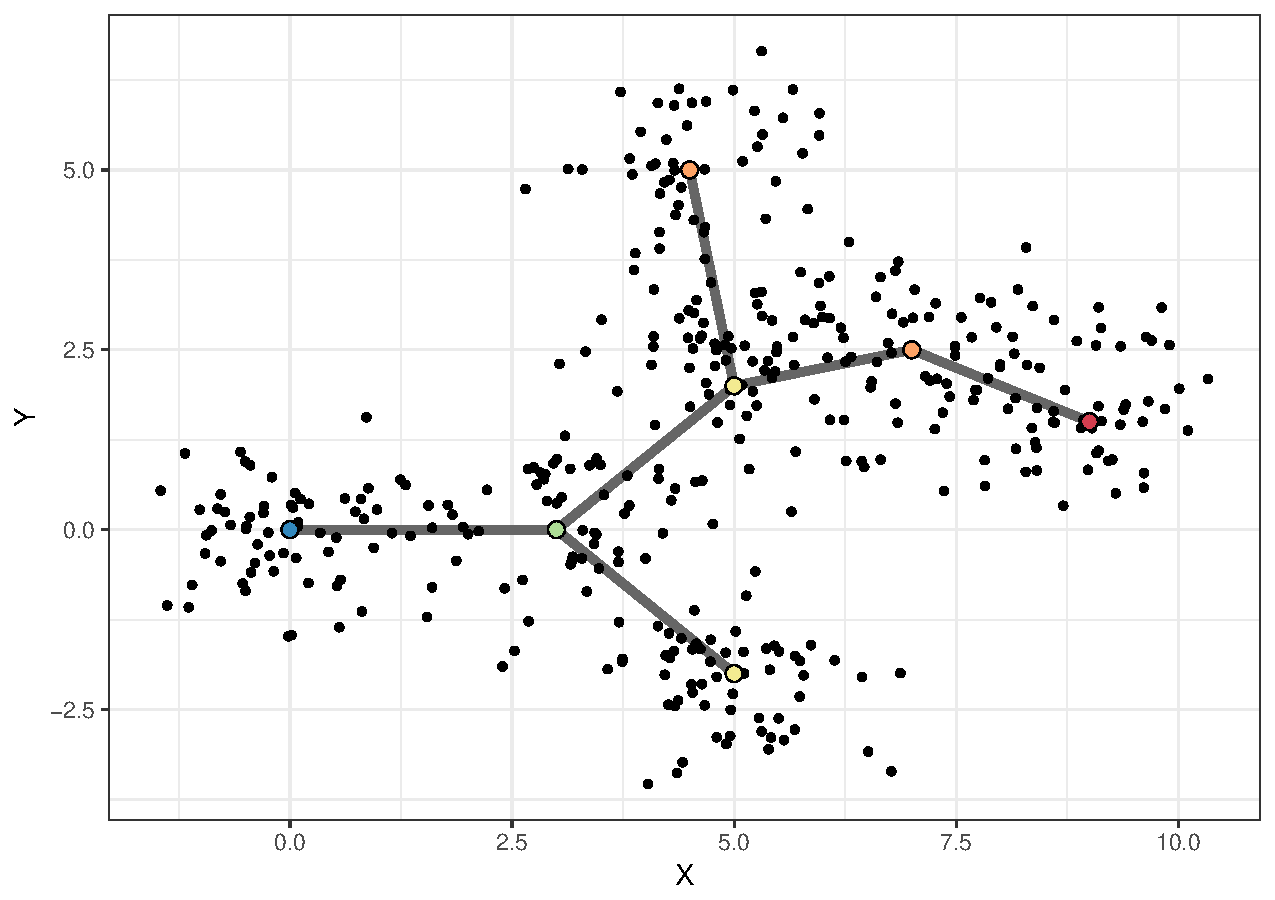
\includegraphics[width=.33\linewidth]{Img/Simulated/true}
    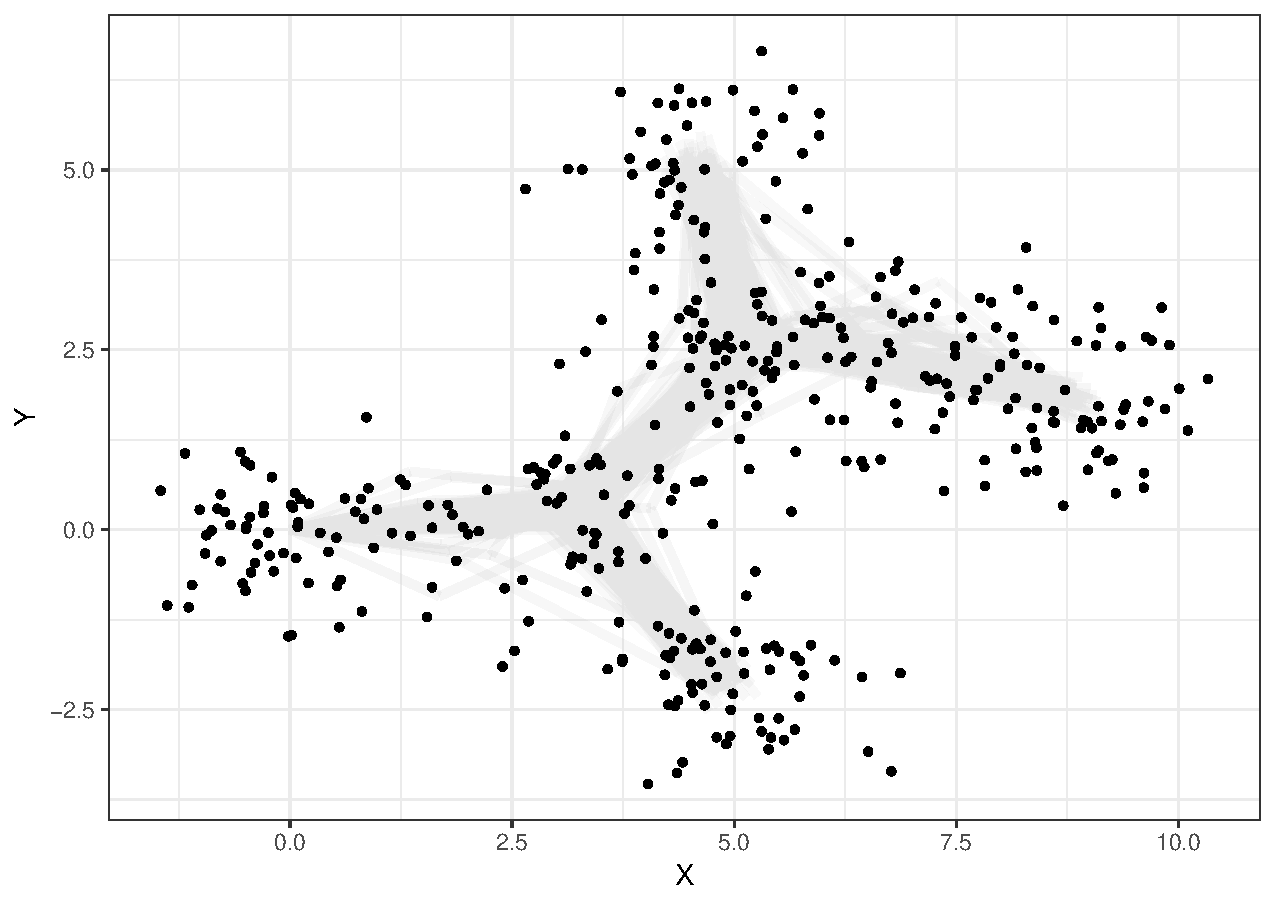
\includegraphics[width=.33\linewidth]{Img/Simulated/posterior_trees}
\caption{Fit of the s-MST model. The left panel shows the simulation
  truth. The right panel shows $M=500$ posterior samples of $\tau_k$.}
\label{fig:sim1_tree}
\end{figure}


\begin{figure}[!ht]
  \centering
    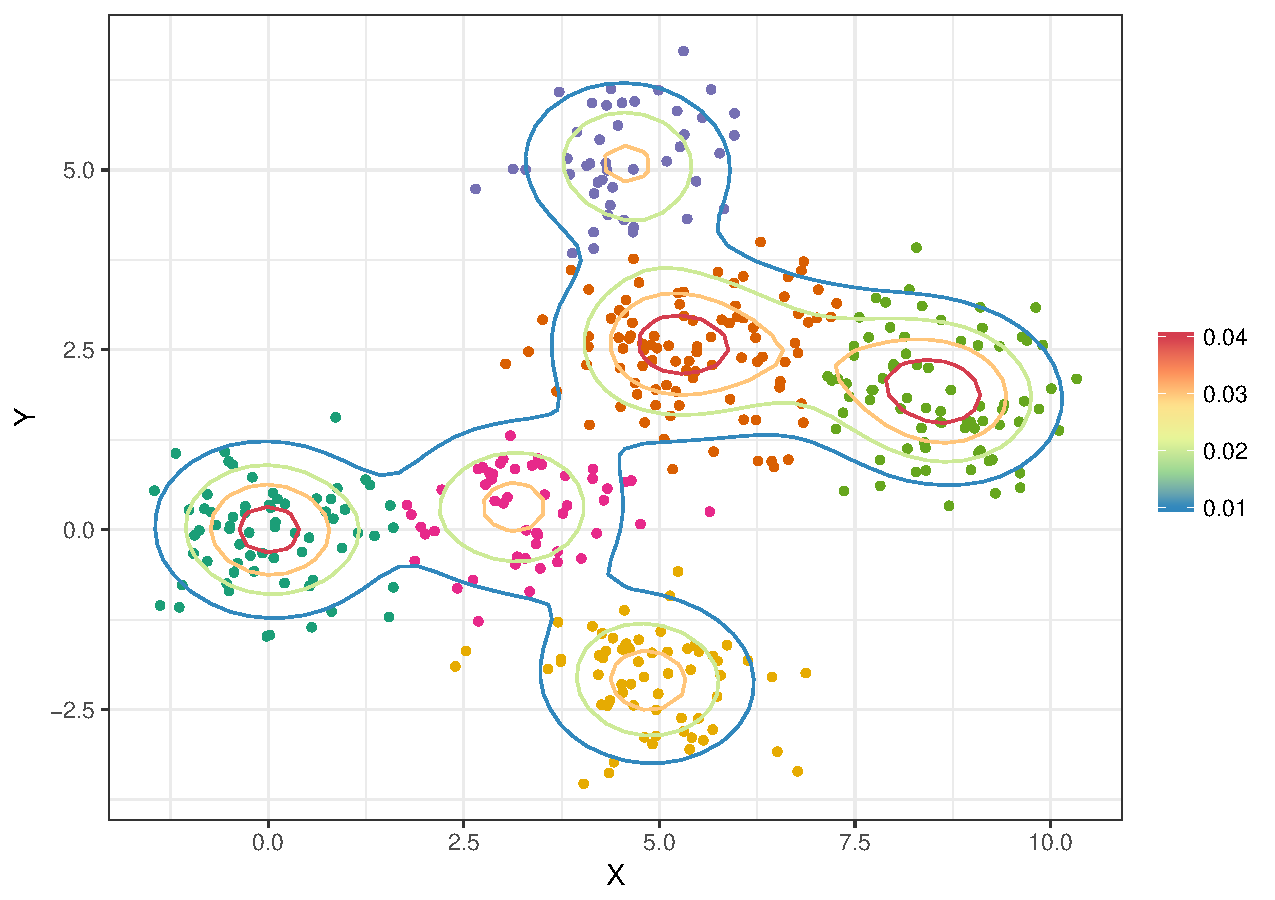
\includegraphics[scale = 0.4]{Img/Simulated/posterior_estimate}
\caption{Posterior density
  estimate obtained via the s-MST model. The observations are colored
  according to the optimal cluster labeling.}
\label{fig:sim1_dens}
\end{figure}


\subsubsection*{Hard MST}

Inference under the h-MST model is done via transdimensional MCMC according to Section \ref{sec:mst_inference} (full conditional distributions are described in Appendix \ref{sec:app_hmst}). First, we run very short parallel MCMC chains (5 iterations) with fixed number of components $k$ ranging from 2 to 15. In this first step, the full conditionals in Appendix \ref{sec:app_hmst} are computed using only the training data and transdimensional moves are not proposed. The second step consists of 10000 iterations of the transdimensional MCMC in which changes in the number of components $k$ are proposed as in Section \ref{sec:mst_inference} followed by the regular Gibbs sampling updates listed in Appendix \ref{sec:app_hmst}. Finally, cluster membership point estimates $\hat{\bfc}:=(\hat{c}_1, \ldots, \hat{c}_n)$ are obtained based on those 10000 iterations following \cite{wade2018bayesian}. Fixing $\bfc = \hat{\bfc}$  (which also implies a fixed posterior estimate on $k$) we run the update steps 2-5 in \ref{sec:app_hmst} for more 5000 iterations. 

Table \ref{tab:k_hmst_sim1} shows the results of the estimation of $k$ under different initial number of mixture components $k_0\in \{2,8,15\}$ and different fractions of training data $\epsilon \in\{0.1, 0.25, 0.5, 0.75\}$ reserved for proposing transdimentional moves. In general, the h-MST favors more parsimonious trees in comparison with the s-MST prior. Here, the results from both soft and hard models are quite similar. The h-MST model recovers 6 clusters for most configurations of $k_0$ and $\epsilon$. Notice how in the simulation, one of the centroids could be "erased" without causing big differences in the underlying tree. The h-MST therefore provided a more parsimonious tree in comparison with the s-MST.

Figure \ref{fig:sim1_multiple_trees_hmst} shows the posterior estimates on the MST structure and cluster membership for $k_0=8$ and $\epsilon=0.5$. The branching structure is well recovered by the h-MST model with six clusters instead of the simulated truth of 7, which was also observed with the s-MST. We can see that using one node less than the in the simulation true, did not compromise the overall branching structure of the tree.

% Table created by stargazer v.5.2.2 by Marek Hlavac, Harvard University. E-mail: hlavac at fas.harvard.edu
% Date and time: Wed, Mar 20, 2019 - 05:17:47 PM
%\begin{table}[!htbp] \centering 
%  \caption{Estimated number of clusters $k$ under the hMST model. The methodology of \cite{wade2018bayesian} was applied to the first 10000 iterations of the transdimensional MCMC under different choices of $\epsilon$ (fraction of data reserved as training) and $k_0$ (value of $k$ used in the initialization of the MCMC algorithm).} 
%  \label{tab:k_hmst_sim1} 
%\begin{tabular}{@{\extracolsep{5pt}} cccc} 
%\\[-1.8ex]\hline 
%\hline \\[-1.8ex] 
% & $k_0=2$ & $k_0=8$ & $k_0=15$ \\ 
%\hline \\[-1.8ex] 
%$\epsilon=0.1$ & $3$ & $6$ & $6$ \\ 
%$\epsilon=0.25$ & $4$ & $6$ & $6$ \\ 
%$\epsilon=0.5$ & $6$ & $6$ & $6$ \\ 
%$\epsilon=0.75$ & $6$ & $6$ & $6$ \\ 
%\hline \\[-1.8ex] 
%\end{tabular} 
%\end{table} 

\begin{table}[!htbp] \centering 
  \caption{Estimated number of clusters $k$ under the hMST model. The methodology of \cite{wade2018bayesian} was applied to the first 10000 iterations of the transdimensional MCMC under different choices of $\epsilon$ (fraction of data reserved as training) and $k_0$ (value of $k$ used in the initialization of the MCMC algorithm).} 
  \label{tab:k_hmst_sim1} 
\begin{tabular}{@{\extracolsep{5pt}} cccc} 
\\[-1.8ex]\hline 
\hline \\[-1.8ex] 
 & $k_0=2$ & $k_0=8$ & $k_0=15$ \\ 
\hline \\[-1.8ex] 
$\epsilon=0.1$ & $3$ & $6$ & $6$ \\ 
$\epsilon=0.25$ & $4$ & $6$ & $6$ \\ 
$\epsilon=0.5$ & $6$ & $6$ & $6$ \\ 
$\epsilon=0.75$ & $6$ & $6$ & $6$ \\ 
\hline \\[-1.8ex] 
\end{tabular} 
\end{table} 



%\begin{figure}[!ht]
%  \centering
%  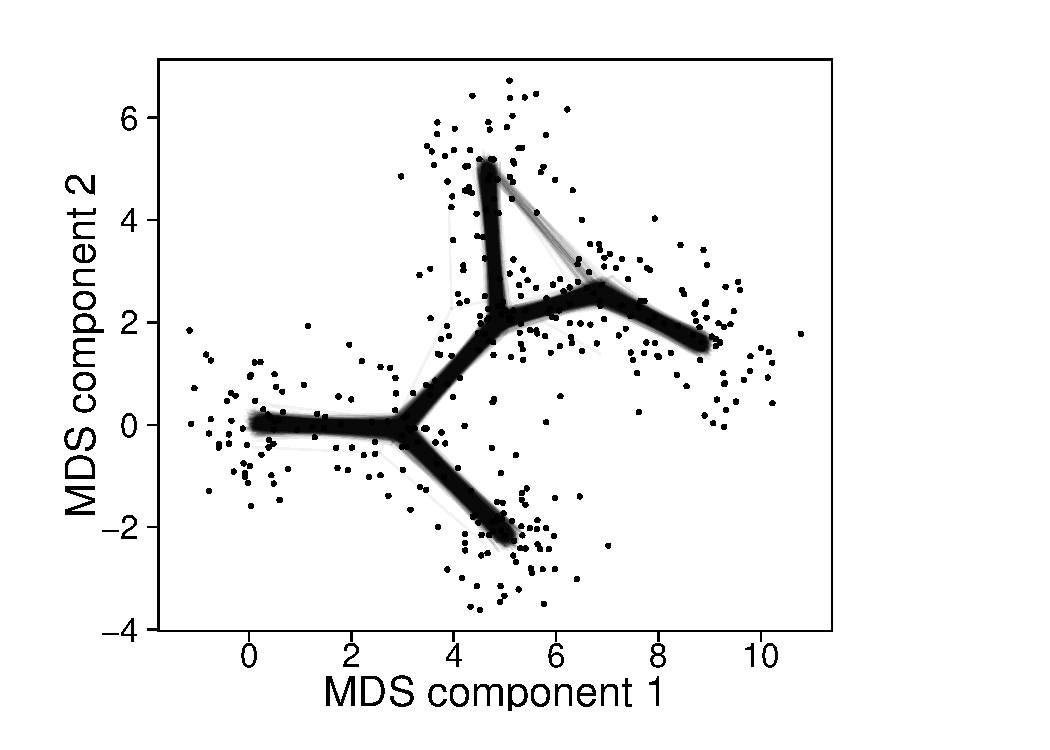
\includegraphics[width=.4\linewidth]{Img/Simulated/multiple_trees_sim1.pdf}
%    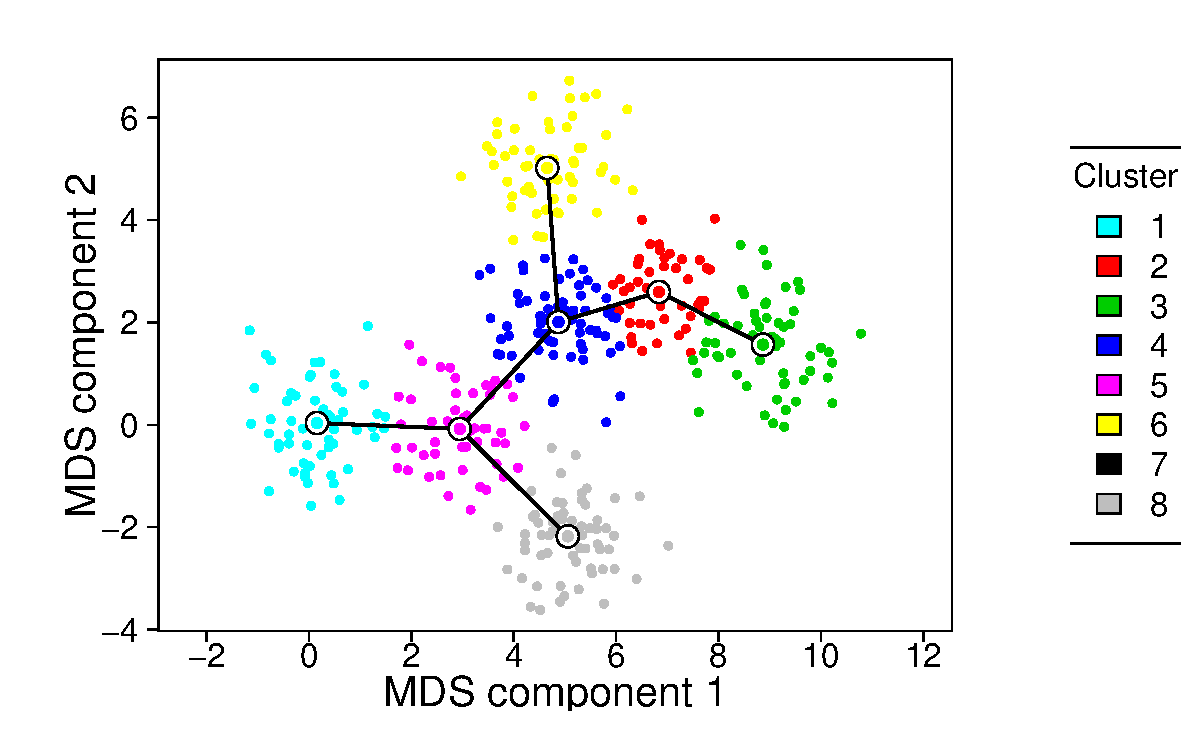
\includegraphics[width=.45\linewidth]{Img/Simulated/sim1_hmst_estimated_tree}
%\caption{Estimated branching structure of the hMST model with $k_0=8$ and $%\epsilon=0.5$ based on the last 5000 MCMC iterations (i.e., cluster membership indicators fixed at posterior estimate). Left panel: stochastic tree estimates under the hMST model. Right panel: multiple runs of slingshot applied to the simulated data.}
%\label{fig:sim1_multiple_trees_hmst}
%\end{figure}


\begin{figure}[!ht]
  \centering
  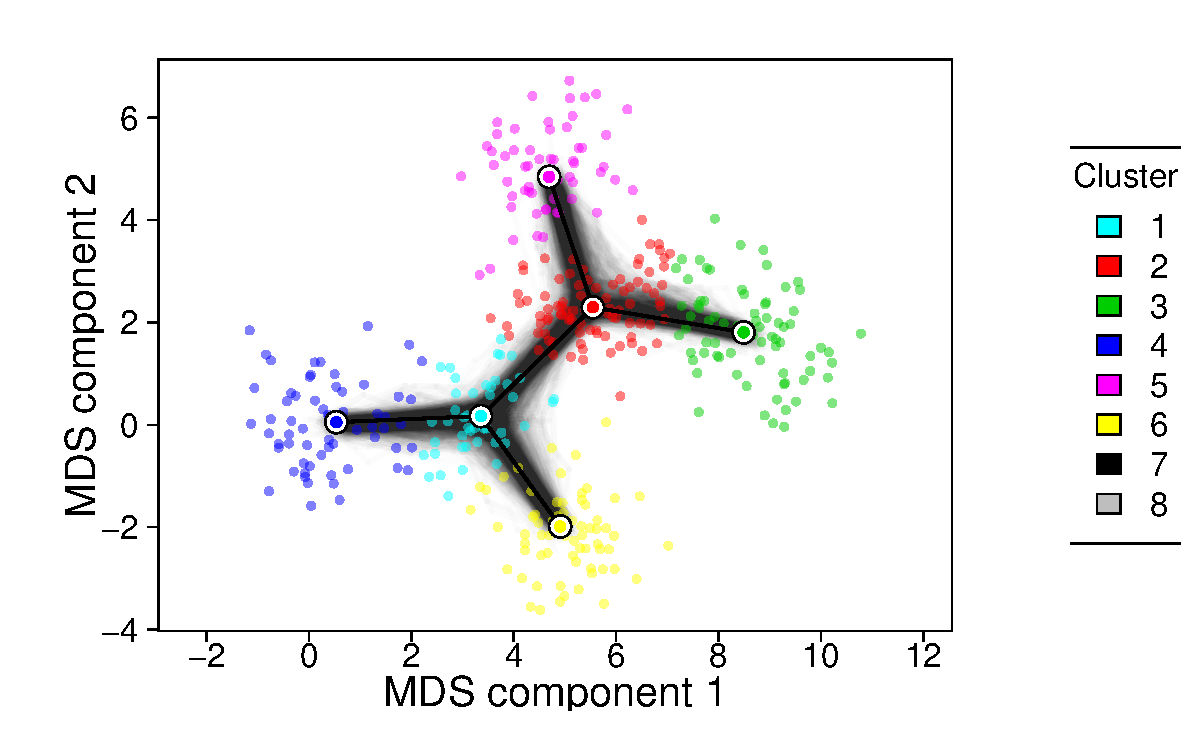
\includegraphics[scale = 0.5]{Img/Simulated/tree_all_in_one.pdf}
\caption{Estimated branching structure of the hMST model with $k_0=8$ and $\epsilon=0.5$ based on the last 5000 MCMC iterations. When the cluster membership indicators are fixed at the point estimate a posteriori, clusters 7 and 8 are empty.}
\label{fig:sim1_multiple_trees_hmst}
\end{figure}



\subsubsection*{Slingshot}

When analyzing the results of applying k-means (k=7) for recovering the clustering of cells followed by the slingshot algorithm to the simulated data, we noticed that some initializations lead to cluster structures that do not correspond to the truth under simulation. This issue is fixed once we consider a higher number of random initializations and select the one with best value of the objective function (Figure \ref{fig:sim1_slingshot_multipleK}). The slingshot algorithm is robust to the choice of $k$, specially when picking large values of $k$ in the k-means algorithm. The method however does not account for statistical uncertanty, which is accomodated in the s-MST and h-MST.

\begin{figure}[H]
  \centering
  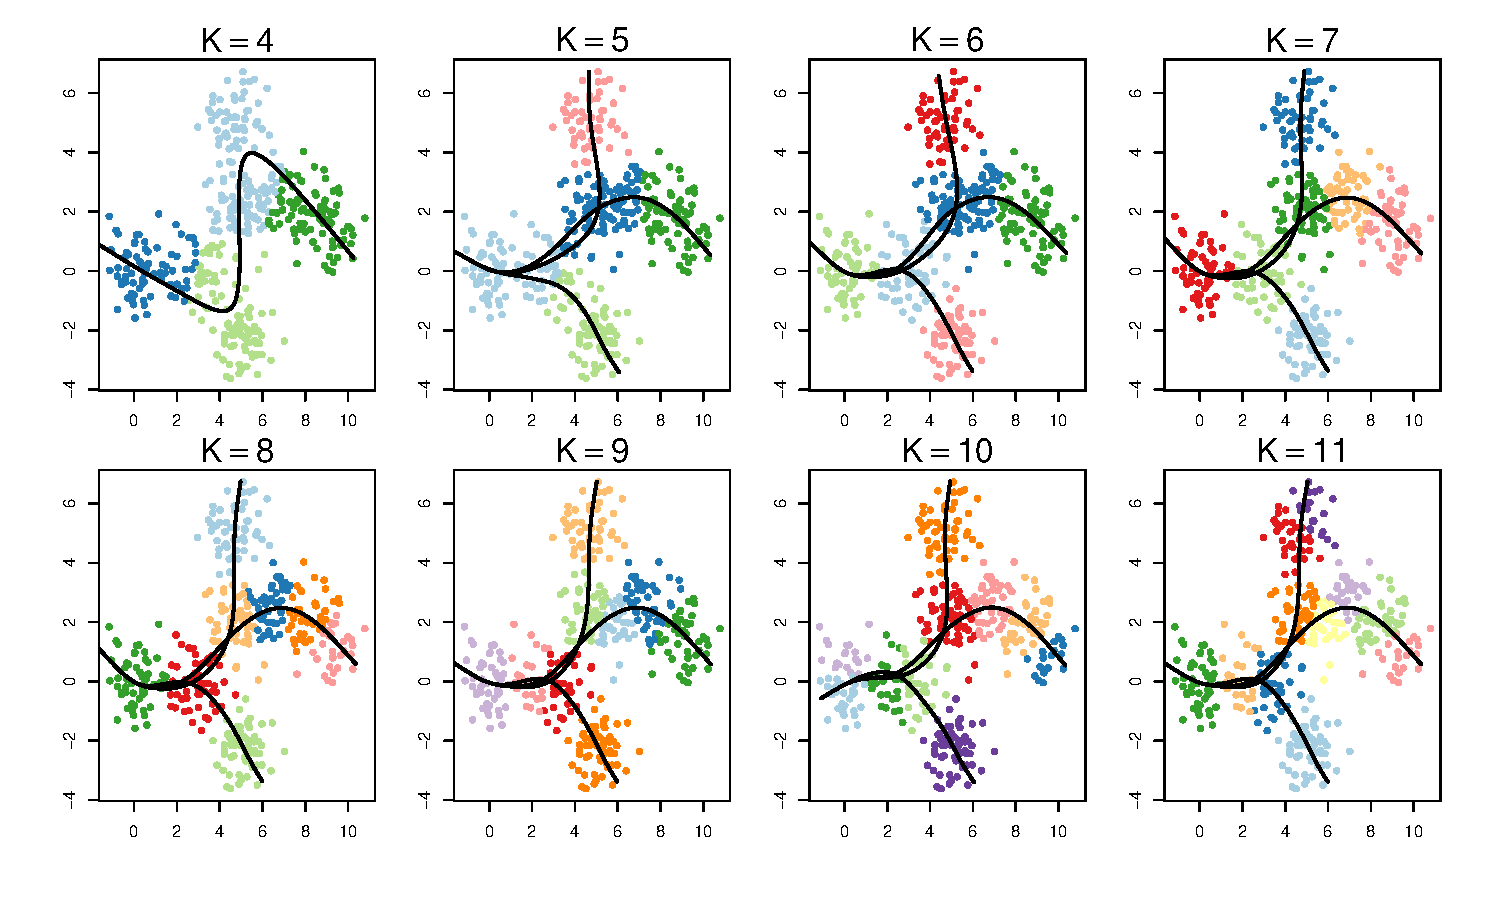
\includegraphics[scale = 0.5]{Img/Simulated/slinghot_sim_1_multipleK_2.pdf}
\caption{Parallel runs of slingshot applied to the simulated data for $k$ ranging from 4 to 11. Clusters are estimated by the best result among 10 random initializations of the k-means algorithm.}
\label{fig:sim1_slingshot_multipleK}
\end{figure}


\subsection{Simulation 2}

We now apply the algorithm to the same simulated dataset presented in
\cite{street2018}.  In Figure \ref{fig:sim2_groups} (left) we show samples from
the posterior on the trees. The density estimate in Figure
\ref{fig:sim2_groups} (right) fits the data well.


\begin{figure}[!ht]
  \centering
  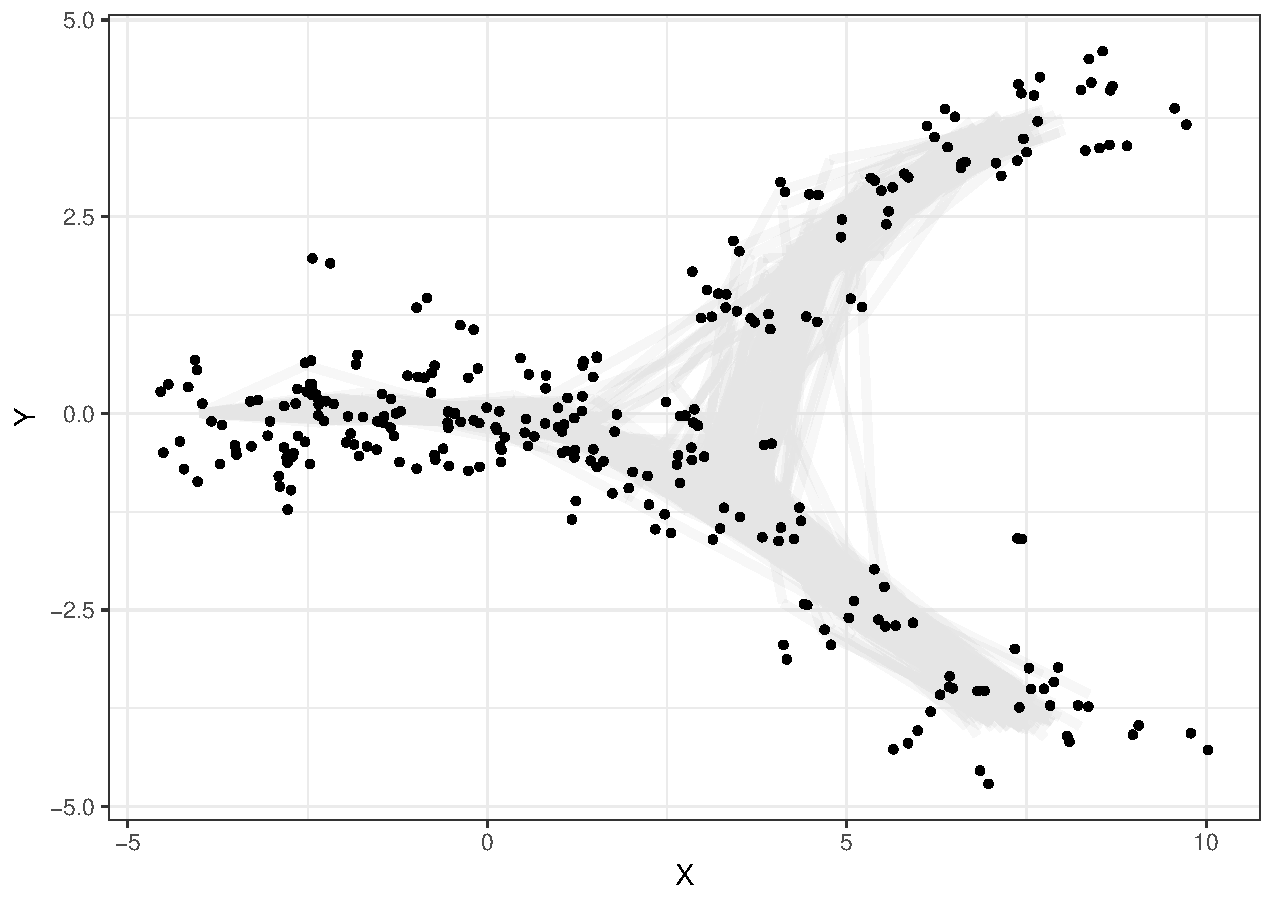
\includegraphics[width=.49\linewidth]{Img/Sim_slingshot/posterior_trees}
  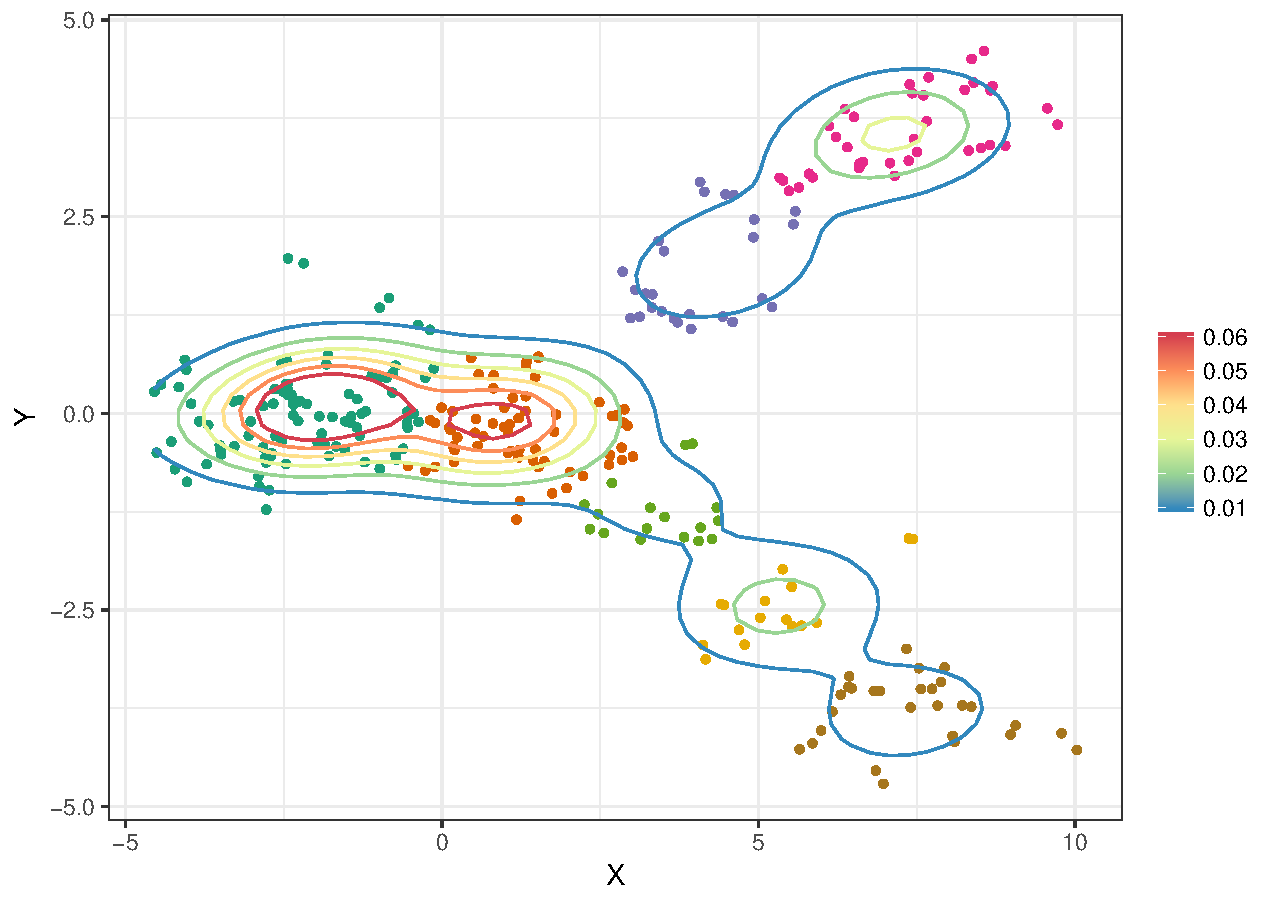
\includegraphics[width=.49\linewidth]{Img/Sim_slingshot/posterior_estimate}
\caption{Left panel: Plot of the posterior sampled trees. Right panel: posterior density estimate obtained via the s-MST model. The observations are colored according to the optimal cluster labeling.}
\label{fig:sim2_groups}
\end{figure}

\subsubsection*{Hard MST}
 
Again, we run 15000 iterations of MCMC on h-MST model. The first 10000 iterations include transdimensional proposal based on splitting the data into training and test, while the last 5000 are evaluated conditionally on the VI point estimate for the cluster membership structure. The h-MST model enforces more parsimony than the s-MST, which can be seen in Figure \ref{fig:sim2_hmst} as fewer components (five) are identified by MCMC.

%\begin{figure}[!ht]
%  \centering
%    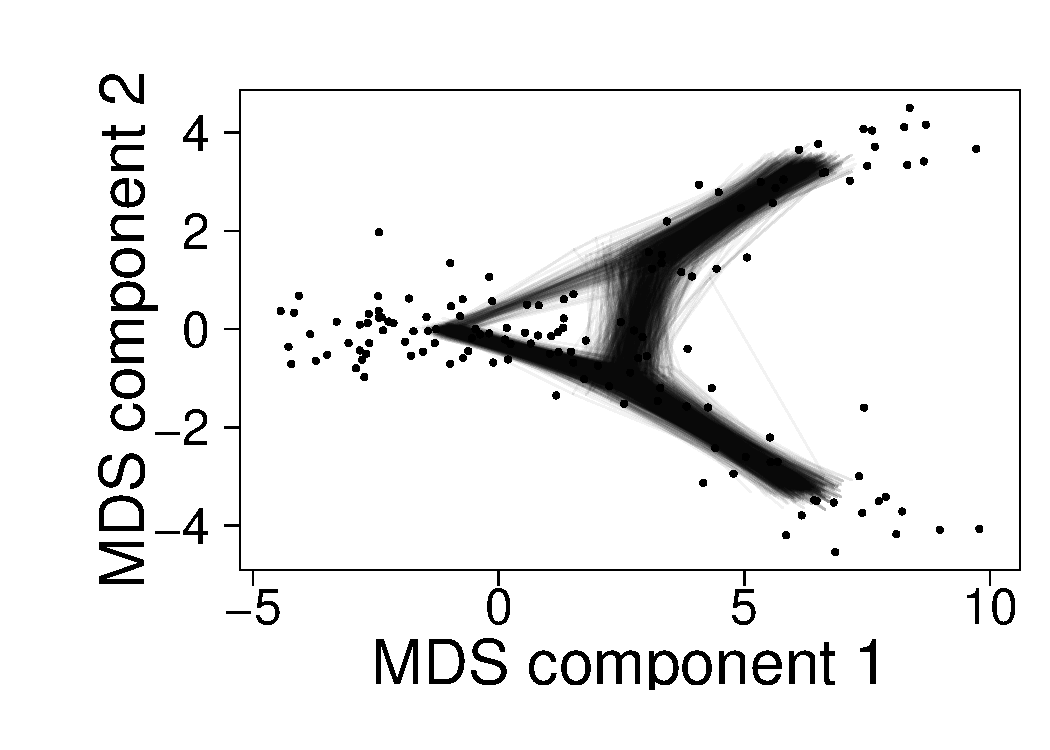
\includegraphics[width=.49\linewidth]{Img/Sim_slingshot/multiple_trees_slingshot_Kinit12.pdf}
%  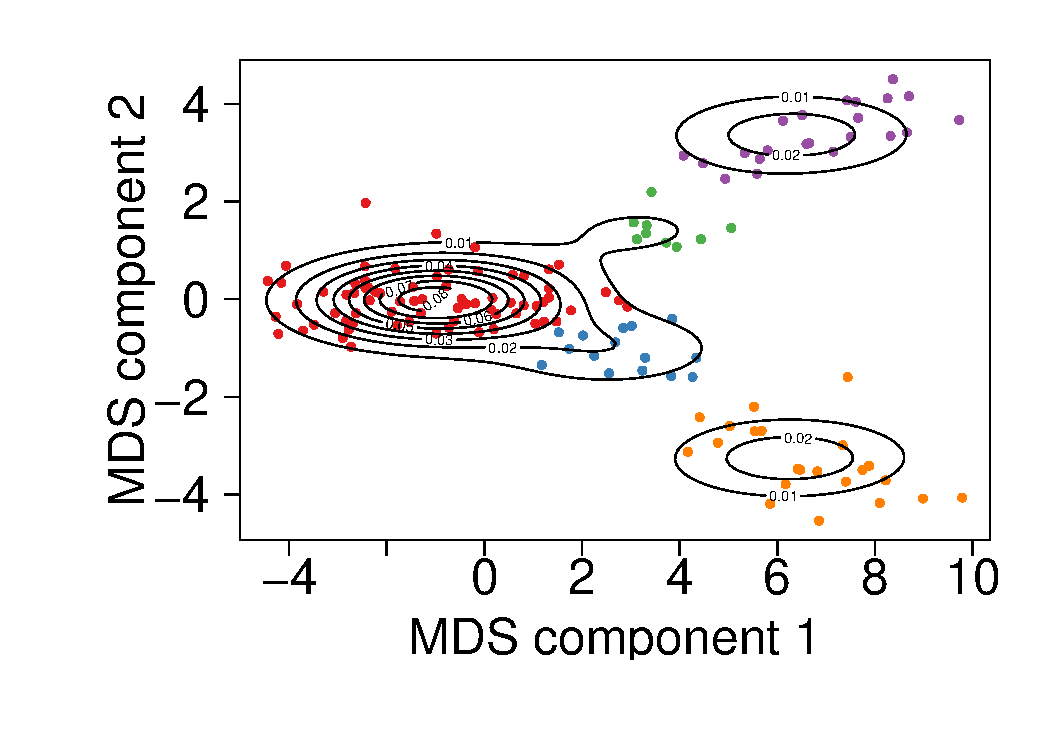
\includegraphics[width=.49\linewidth]{Img/Sim_slingshot/posterior_density_Kinit_12.pdf}
%\caption{Left panel: Sampled MST given the cluster membership estimates. Right panel: posterior density estimate obtained via the h-MST model. The observations are colored according to the optimal cluster labeling.}
%\label{fig:sim2_hmst}
%\end{figure}

\begin{figure}[!ht]
  \centering
  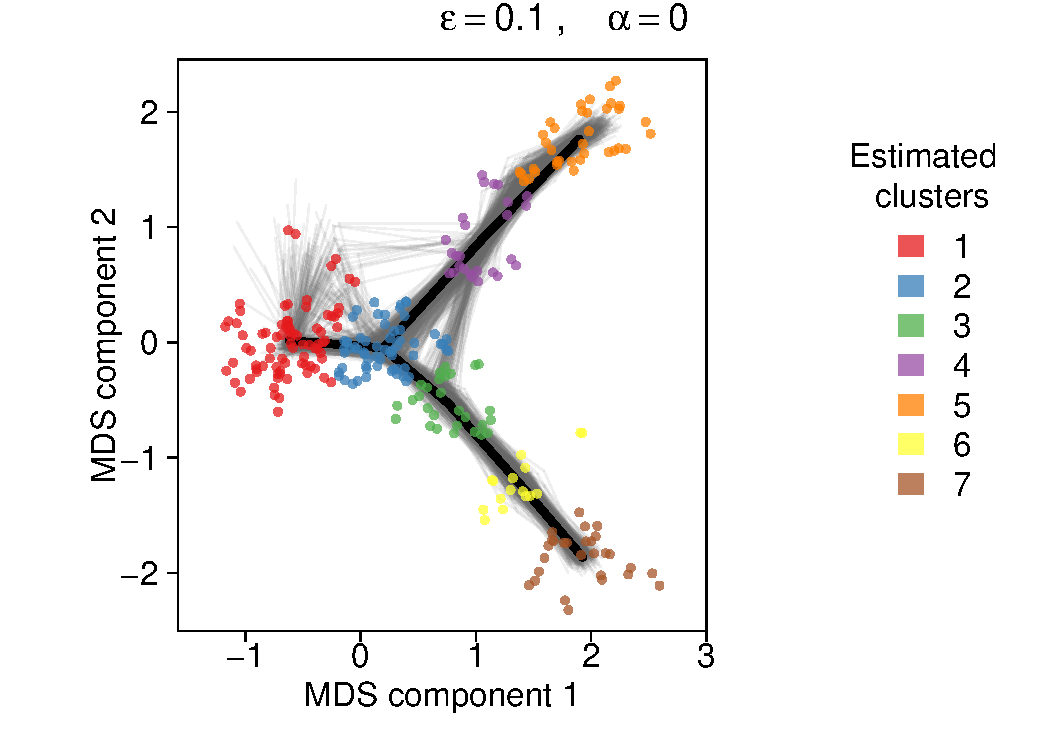
\includegraphics[width=.48\linewidth]{Img/Sim_slingshot/estimated_trees_slingshot_eps_01_xi_0.pdf}
  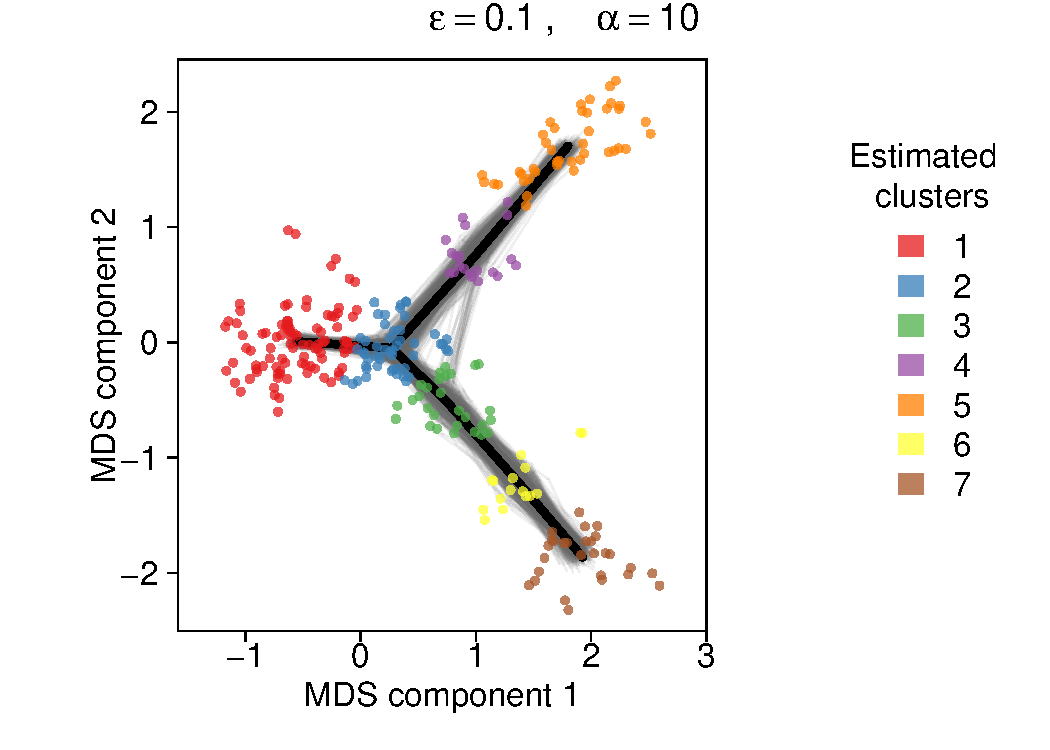
\includegraphics[width=.48\linewidth]{Img/Sim_slingshot/estimated_trees_slingshot_eps_01_xi_10.pdf}
\caption{Results of posterior estimation of MST. Curves in gray are the posterior sampled MST and the black tree in the point estimate a posteriori. $\alpha$ represents the strength of regularization towards simple MST structures that is implied by the hMST prior on $\bfmu$. $\epsilon$ is the fraction of the data reserved as training for the purpose of building the transdimensional proposals.}
\label{fig:sim2_hmst}
\end{figure}



\section{Mouse Data}

We  analyze data from 
a single cell RNA-seq experiment on horizontal basal cells (HBC) from the adult mouse
olfactory epithelium \citep{street2018}.
The goal is to infer the continuous progression from stem cells into
terminal mature cells and to estimate the cell-specific pseudotimes.

Due to the heterogeneity of cell populations, the analysis of
traditional transcription data, such as bulk microarrays, does not
allow researchers to discover cell dynamics. In fact, the underlying
signal can be potentially masked when averaging over thousands of
samples \citep{korthauer2016statistical},  possibly compromising
statistical power. 

The original data (before preprocessing) is available on GEO in
GSE95601 and also in
https://github.com/drisso/fletcher2017data. Preprocessing follows the steps in \citep{perraudeau2017}, which are listed here for completeness. The dataset originally contains measurements for 28284 genes throughout 849 cells. A total of 102 low-quality cells are removed from the dataset and the 1000 most variable genes are retained.

The resulting data is then normalized and the dimension is further
reduced to 50 by fitting a Zero-Inflated Negative Binomial-based Wanted Variation Extraction (ZINB-WaVE) model following \cite{zinbwave}. The ZINB-WaVE assumes a zero inflated negative bionomial model to extract low-dimensional signal from the data, accounting for dropouts (inflation of zeros), over-dispersion, and the count nature of the single cell RNA-seq data. Finally, multidimension scale (MDS) \citep{mardia1979} is applied to reduce the dimension further to 2 (this is the only deviation from \citealt{perraudeau2017} in which the dimension is reduced to 5). MDS consists of a rearrangement of the observations in a lower dimensional space (dimension 2 here) based on the matrix of pairwise distances computed using all the original 50 dimensions.

\paragraph*{Hard-MST model.}
We start by showing results of application of the model that enforces
MST structure (Section \ref{sec:model2_mst}). The RJMCMC was run for
3000 iterations. The first 2000 are used to obtain a point
estimate for the cluster membership indicators $c_i$ according with
\cite{dahl2006} and also for the number of mixture components
$k$. The final 1000 iterations are run with fixed $c_i$ and $k$.
The hyperparameters were chosen as $r_0 = 0.5$, $a_0=b_0=10$,
$\sigma^2_0=1$, $\lambda_0=1$ and $\delta=1$ to reflect
non-informative prior knowledge.


Figure \ref{fig:fletcher_est_tree} shows the estimation of the underlying minimum spanning tree. We estimate 8 nodes with one branching leaving the main path of the spanning tree (green). The right pannel illustrates the posterior uncertainty on the edges of the tree and highlights the proximity of green cluster with both the purple and the yellow clusters.


\begin{figure}[!ht]
  \centering
  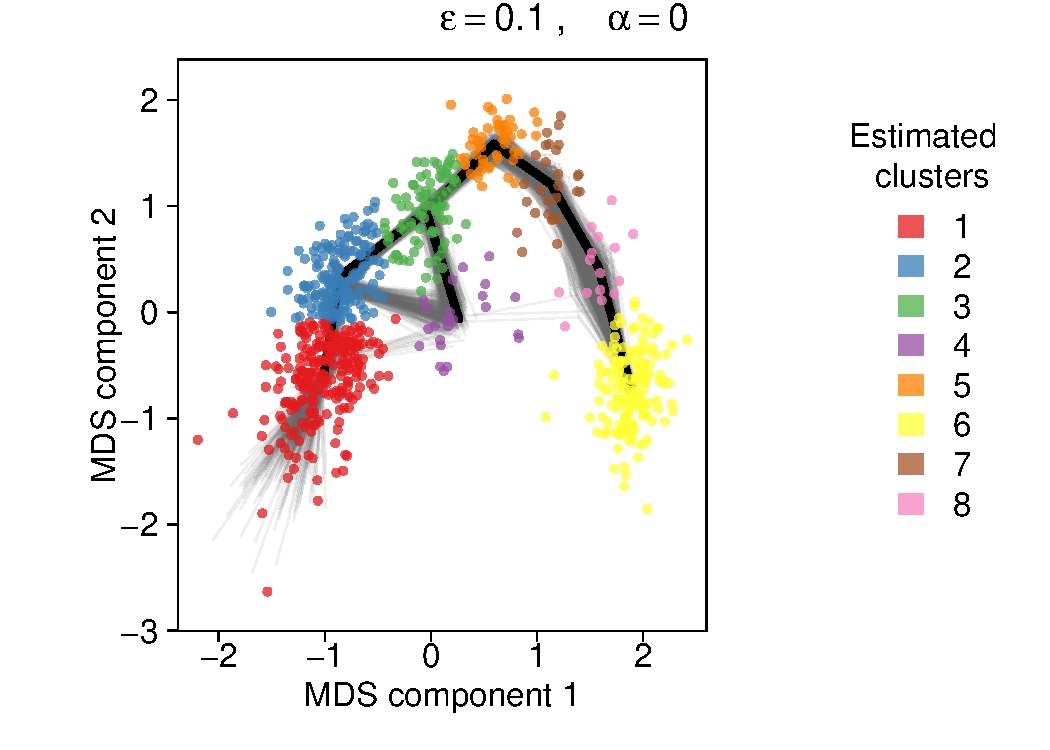
\includegraphics[width=.49\linewidth]{./Img/fletcher/estimated_trees_slingshot_eps_01_xi_0.pdf}
  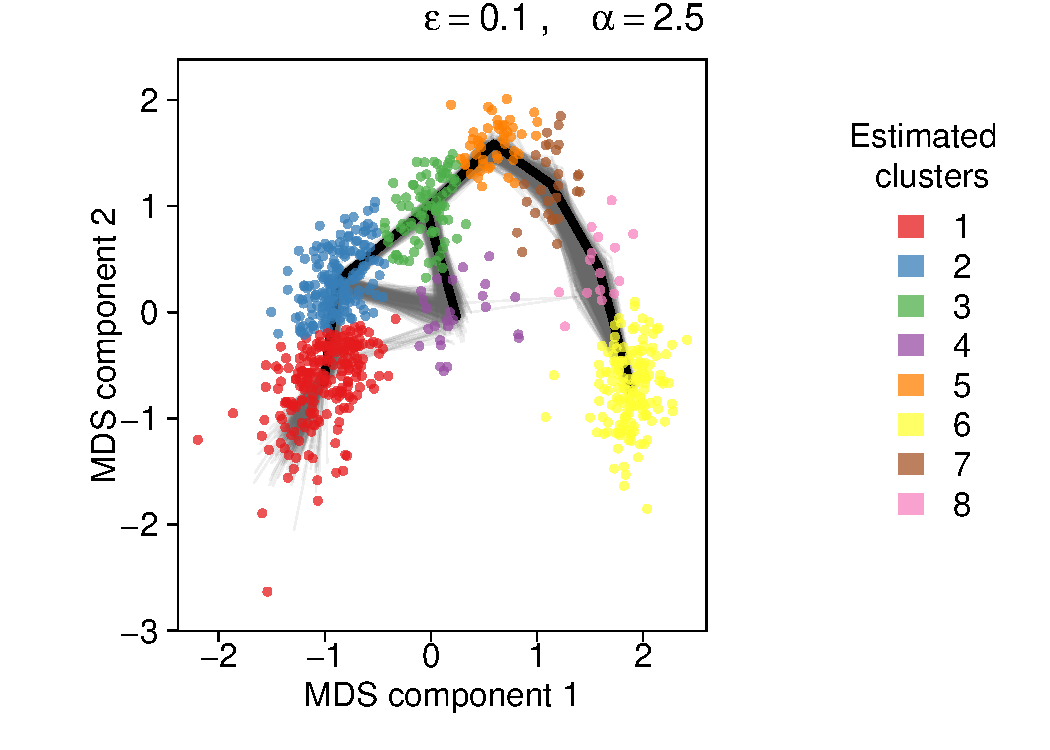
\includegraphics[width=.49\linewidth]{./Img/fletcher/estimated_trees_slingshot_eps_01_xi_25.pdf}
\caption{Posterior estimates of the latent MST and clustering membership structure based on the last 5000 MCMC iterations. Left panel: independent mixture ($\alpha = 0$). Right panel: MST dependent mixture ($\alpha=2.5$).}
\label{fig:fletcher_est_tree}
\end{figure}



We now focus on posterior estimation of pseudotimes. For each MCMC
sample (after burn-in) we construct a posterior sample for the
cell-specific pseudotimes as a deterministic transformation 
of the underlying MST. Such transformation is defined by calculating the
distance along the tree from its root node to the projection of the
cell onto the closest edge in the tree. 
 Let $T_i(\tau)$ denote the pseudotime for cell $i$. 
Figure \ref{fig:fletcher_est_pseudo}a
illustrates the evaluation of $T_i(\tau)$, 
where the
particular tree in the plot is fixed as the MST $\tau$ determined by the
posterior point estimates for the cluster centers. 
The right panel shows marginal posterior standard deviations for the
cell-specific pseudotimes,  conditional on cluster membership. 
Such graphical summaries help to identify those cells
that are more prone to missclassification for being at approximately
equal distance from two or more branches in the MST. 

%Figure \ref{fig:fletcher_hist}  shows the histogram of pseudotimes for cell
%707 (the one marked in black in Figure \ref{fig:fletcher_est_pseudo})
%in comparison with a typical cell from the green cluster (e.g, 730)
%and also from the black cluster (e.g., 631, 632). The small local mode
%near 0.1 indicates the proximity of cell 707 from those in cluster 2
%(black) and explains the high variance of its pseudotime a posteriori. 

\begin{figure}[!ht]
  \centering
  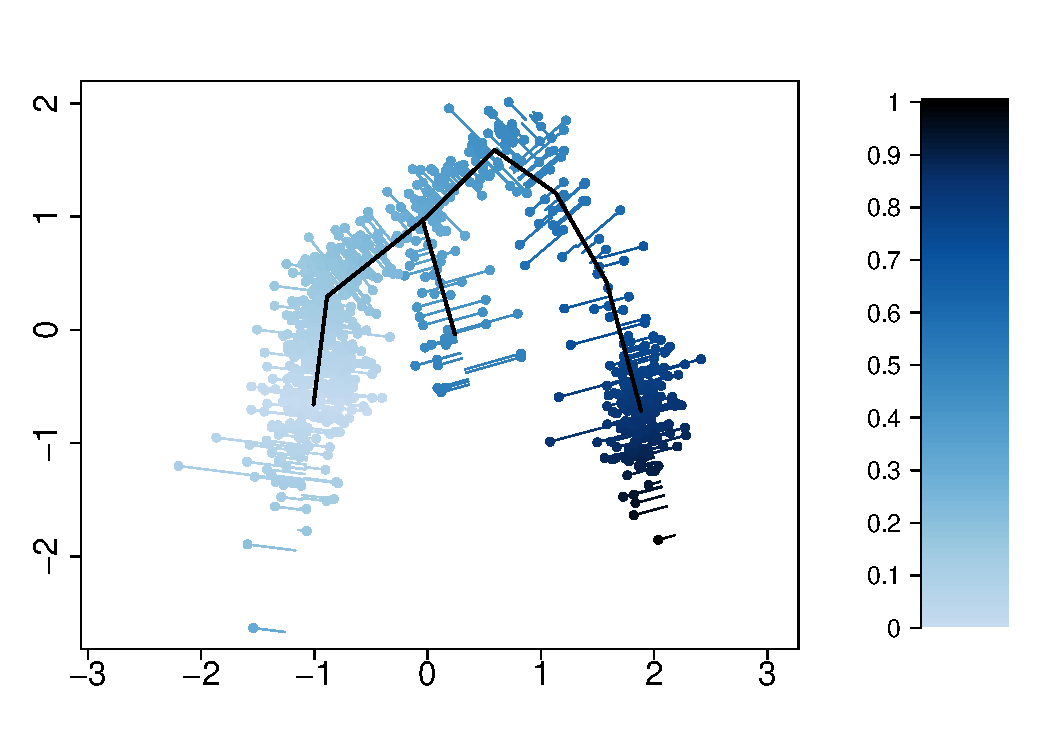
\includegraphics[width=.49\linewidth]{Img/fletcher/estimated_pseudotime_new.pdf}
  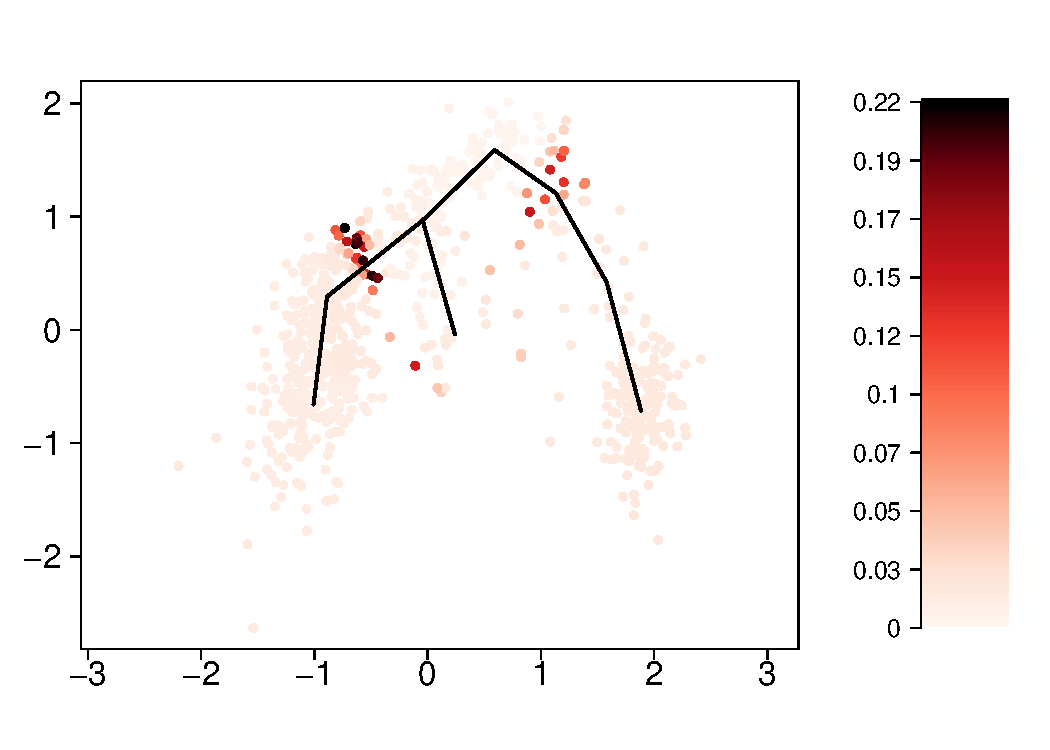
\includegraphics[width=.49\linewidth]{Img/fletcher/sd_pseudotime_new.pdf}
\caption{Left panel: Estimated pseudotimes for each cell. The extremes
  0 and 1 were chosen arbitrarily. 
  Right panel: posterior standard deviation of pseudotimes for each cell. Axis represent the two components of the MDS transformation.}
\label{fig:fletcher_est_pseudo}
\end{figure}


%\begin{figure}[!ht]
%  \centering
%  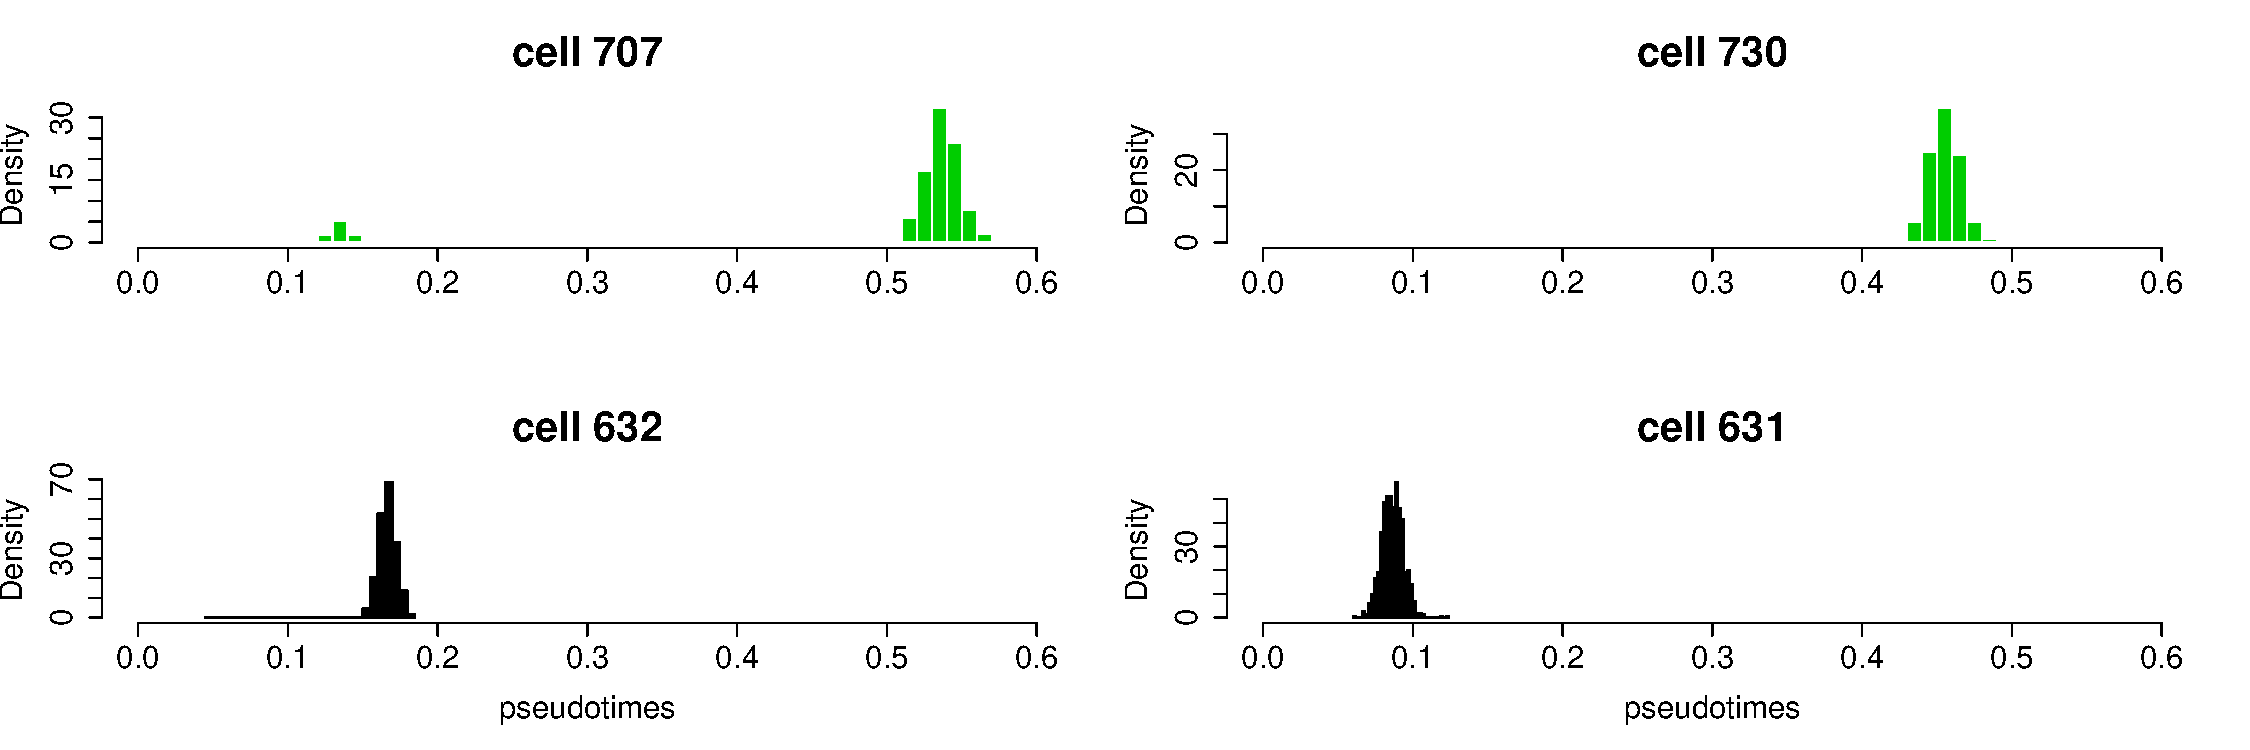
\includegraphics[scale = 0.4]{Img/fletcher/histograms.pdf}
%\caption{Posterior pseudotime distributions for two cells in clusters 2 and 5. }
%\label{fig:fletcher_hist}
%\end{figure}


In Figure \ref{fig:fletcher_boxplot}, we can have a broader view of
the estimated pseudotimes for cells in each one of the $k$ clusters. 

\begin{figure}[!ht]
  \centering
  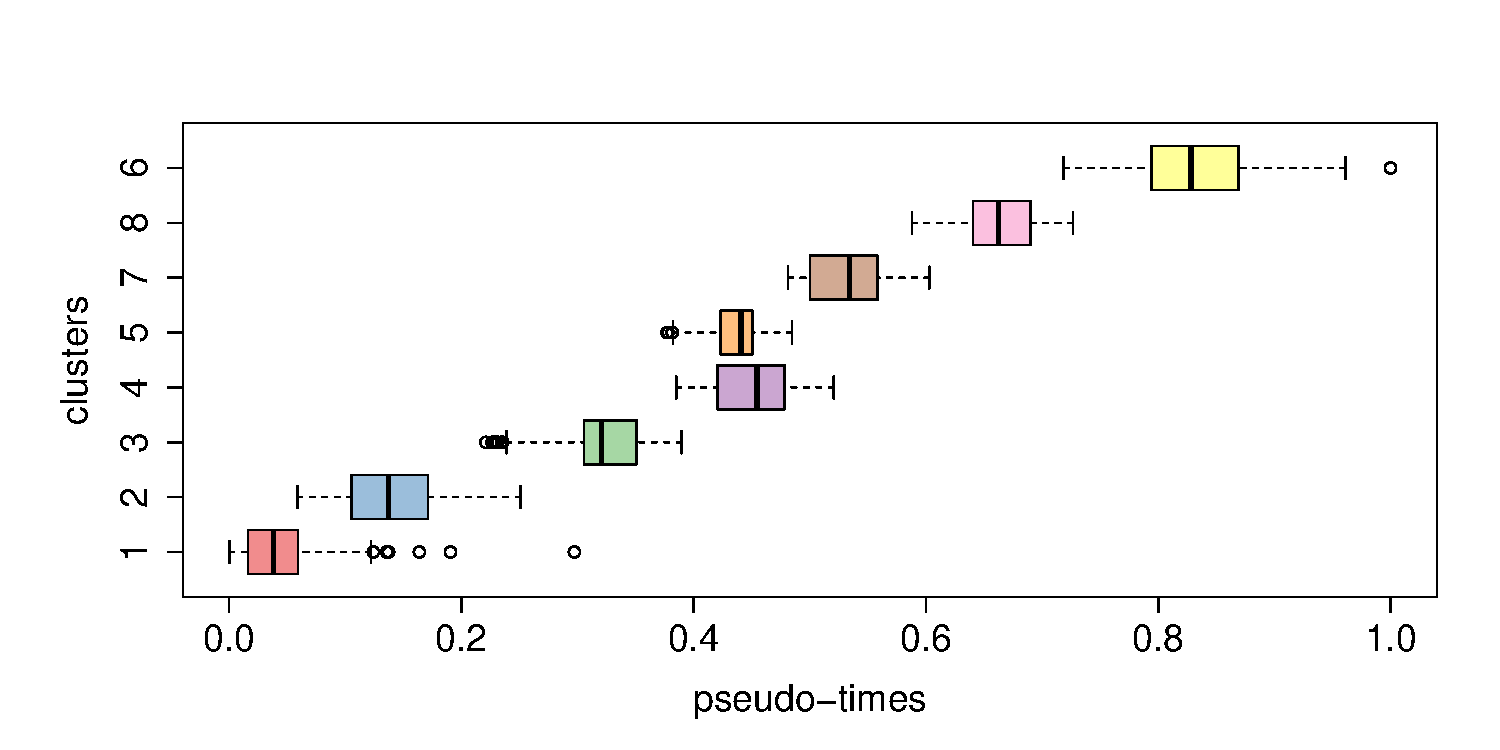
\includegraphics[scale = 0.4]{Img/fletcher/bp_pseudotime_new.pdf}
\caption{Cluster specific boxplots of median posterior pseudotimes obtained for each cell.}
\label{fig:fletcher_boxplot}
\end{figure}

\paragraph*{Slingshot.} The slingshot method is a multistep algorithm that produces an underlying MST conditional on a fixed estimate of the cluster centroids. The algorithm first computes the MST with the clusters' centroids as nodes. Then it fits for each leaf a principal curve that smooths the path from the root to that leaf along the corresponding branches of the MST. Each principal curve represents a cell different development path.

We now investigate the sensitivity of the slingshot method to the clustering of cells. We apply multiple independent runs of k-means algorithm initialized at random with k=8. Figure \ref{fig:fletcher_slingshot_kmeans} shows that the resulting MST is highly dependent on the initialization of the k-means algorithm, in some cases omitting important branches or creating artificial branches that clearly do not correspond to distinct cell populations. However, picking the best among multiple consistently solves the issue, as illustrated in Figure \ref{fig:fletcher_slingshot_kmeans2}.

\begin{figure}[H]
  \centering
  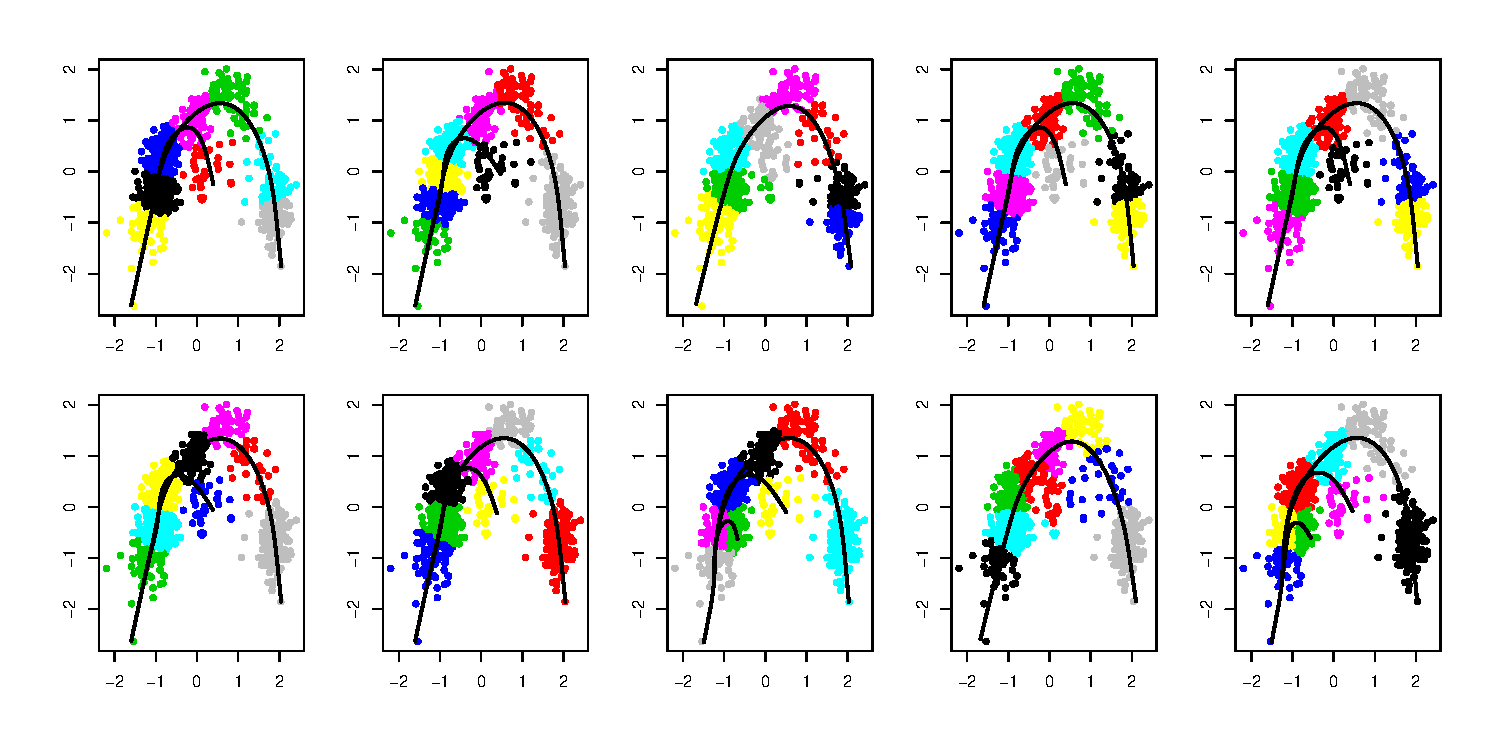
\includegraphics[scale = 0.55]{Img/fletcher/slinghot_estimates.pdf}
\caption{Multiple runs of slingshot applied to the mouse data. Each plot corresponds to a distinct random initialization of k-means algorithm (k=8). Axis represent the 2 MDS components for dimension reduction.}
\label{fig:fletcher_slingshot_kmeans}
\end{figure}

\begin{figure}[H]
  \centering
  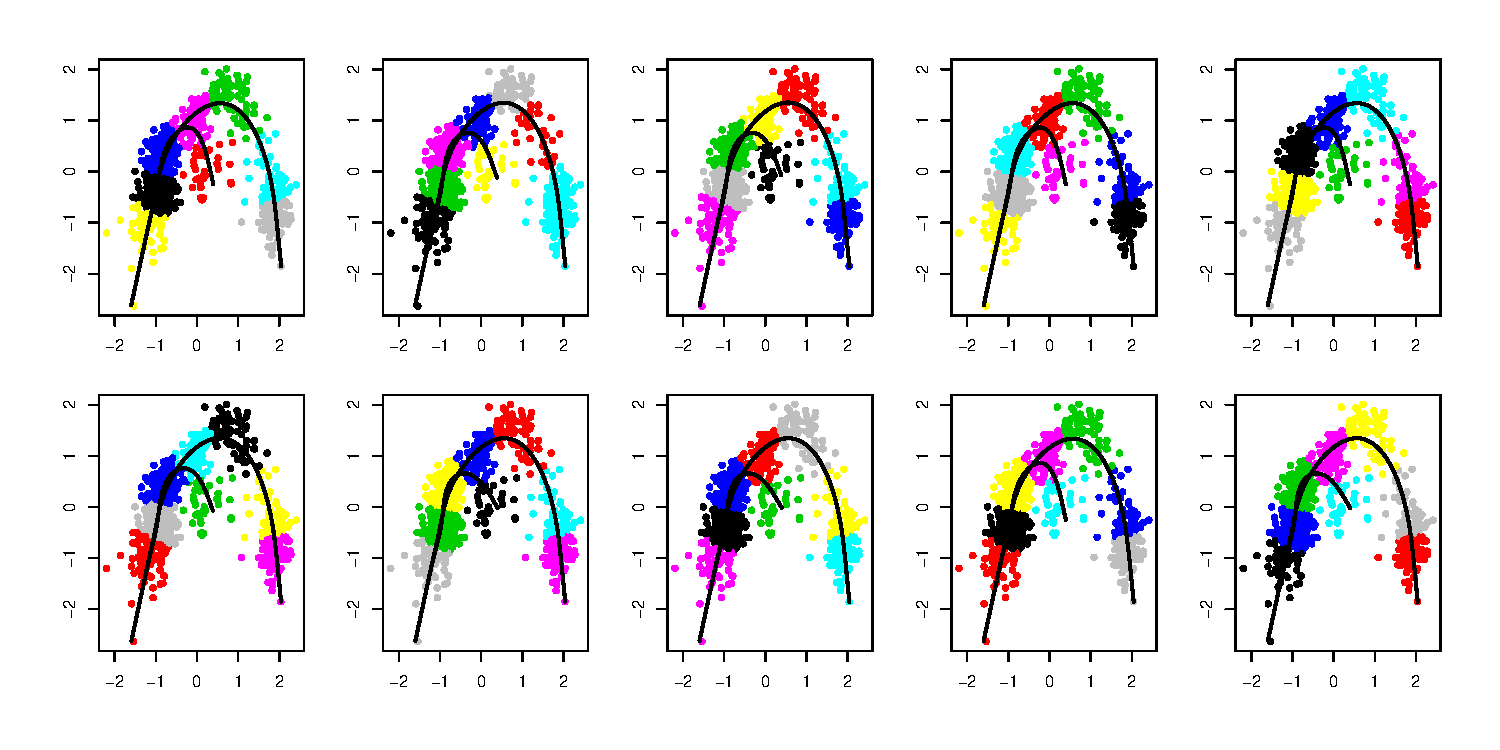
\includegraphics[scale = 0.55]{Img/fletcher/slinghot_estimates_rep.pdf}
\caption{Multiple runs of slingshot applied to the mouse data. Each plot corresponds to the best result among 10 distinct random initializations of k-means algorithm (k=8). Axis represent the 2 MDS components for dimension reduction.}
\label{fig:fletcher_slingshot_kmeans2}
\end{figure}

\section{Discussion}

We developed a dependent mixture model for single cell RNA sequencing data to estimate cell lineages. The proposed model takes into account the underlying tree in the transformed data on a lower dimension when defining the cluster structure of the cells: the model penalizes cluster allocations that define over complex trees. We presented two forms of defining such penalization terms: under soft MST or hard MST.

Motivated by the cell lineage applicaion, we deffined a dependent prior based on tree alignment. Other applications might give rise to dependence based on alignment of clusters on other, more general graphs.





 